\documentclass[
    % MENDT6 item 2
	% -- opções da classe memoir --
	12pt,				% tamanho da fonte
	openright,			% capítulos começam em pág ímpar (insere página vazia caso preciso)
	oneside,			% [oneside or twoside]para impressão em recto e verso. Oposto a oneside (acordo MENDT6 é opcional 1 ou 2 lados, prefenrencialmente 2 lados)
	a4paper,			% tamanho do papel. 
	% -- opções da classe abntex2 --
	chapter=TITLE,		% títulos de capítulos convertidos em letras maiúsculas
	%section=TITLE,		% títulos de seções convertidos em letras maiúsculas
	%subsection=TITLE,	% títulos de subseções convertidos em letras maiúsculas
	%subsubsection=TITLE,% títulos de subsubseções convertidos em letras maiúsculas
	% -- opções do pacote babel --
	english,			% idioma adicional para hifenização
	french,				% idioma adicional para hifenização
	%spanish,			% idioma adicional para hifenização
	brazil				% o último idioma é o principal do documento
	]{abntex2}

% ---
% Pacotes básicos 
% ---
\usepackage{lmodern}			% Usa a fonte Latin Modern			
\usepackage[T1]{fontenc}		% Selecao de codigos de fonte.
\usepackage[utf8]{inputenc}		% Codificacao do documento (conversão automática dos acentos)
\usepackage{indentfirst}		% Indenta o primeiro parágrafo de cada seção.
\usepackage{color}				% Controle das cores
\usepackage{graphicx}			% Inclusão de gráficos
\usepackage{microtype} 			% para melhorias de justificação
% ---
	
% ---
% Pacotes adicionais, usados apenas no âmbito do Modelo Canônico do abnteX2
% ---
\usepackage{amsfonts}
\usepackage{amssymb} 
\usepackage{amsthm}
\usepackage{amsmath}
\usepackage{bm}
\usepackage{comment}
\usepackage{enumerate}

%\usepackage{lipsum}				% para geração de dummy text
\usepackage{tikz}
\usetikzlibrary{positioning}
\usepackage{xcolor}
\usepackage{array}     % Elementos extras para formatação de tabelas

% ---

% ---
% Pacotes de citações
% ---
\usepackage[brazilian,hyperpageref]{backref}	 % Paginas com as citações na bibl
% MENDT6 - podem ser númerica ou autor/data
\usepackage[num]{abntex2cite}	% Citações padrão ABNT 
%\usepackage[alf]{abntex2cite}	% Citações padrão ABNT 

% --- 
% CONFIGURAÇÕES DE PACOTES
% --- 
% Configurações do pacote backref
% Usado sem a opção hyperpageref de backref
\renewcommand{\backrefpagesname}{Citado na(s) página(s):~}
% Texto padrão antes do número das páginas
\renewcommand{\backref}{}
% Define os textos da citação
\renewcommand*{\backrefalt}[4]{
	\ifcase #1 %
		Nenhuma citação no texto.%
	\or
		Citado na página #2.%
	\else
		Citado #1 vezes nas páginas #2.%
	\fi}%

% ------------------------------------------------------------------------
% Informações de dados para CAPA e FOLHA DE ROSTO
% Preenchimento obrigatório

% ---
% Informações de dados para CAPA e FOLHA DE ROSTO
% ---
\titulo{Modelos Analíticos de Segurança Cibernética}
\autor{Vilc Queupe Rufino}
\local{Rio de Janeiro, Brasil}
\data{2019, v-1.0.0}
\orientador[D.Sc.]{Daniel Sadoc Menasché}
\coorientador[D.Sc.]{Josefino Cabral Melo Lima}
\instituicao{%
    Universidade Federal do Rio de Janeiro -- UFRJ
    \par
    Instituto de Matemática
    \par
    Instituto Tércio Pacitti de Aplicações e Pesquisas Computacionais
    \par
    Programa de Pós-Graduação em Informática}
\tipotrabalho{Tese (Doutorado)}
% O preambulo deve conter o tipo do trabalho, o objetivo, 
% o nome da instituição e a área de concentração 
\preambulo{Qualificação de Doutorado a ser submetida à banca de Corpo Docente selecionada pelo Programa de Pós-Graduação em Informática, Instituto Tércio Pacitti de Aplicações e Pesquisas Computacionais, instituto de Matemática da Universidade Federal do Rio de Janeiro. Área de Concentração Informática.}
% ---
% ------------------------------------------------------------------------

% ------------------------------------------------------------------------
% informações do PDF
\makeatletter
% informações do PDF

\hypersetup{
     	%pagebackref=true,
		pdftitle={\@title}, 
		pdfauthor={\@author},
    	pdfsubject={\imprimirpreambulo},
	    pdfcreator={LaTeX with abnTeX2},
		pdfkeywords={epidemia}{rede de computadores}{segurança da informação}{atacante estratégico}{qualificação}, 
		colorlinks=true,       		% false: boxed links; true: colored links
    	linkcolor=blue,          	% color of internal links
    	citecolor=blue,        		% color of links to bibliography
    	filecolor=magenta,      		% color of file links
		urlcolor=blue,
		bookmarksdepth=4
}
\makeatother
% ------------------------------------------------------------------------
 
% ---
% Posiciona figuras e tabelas no topo da página quando adicionadas sozinhas
% em um página em branco. Ver https://github.com/abntex/abntex2/issues/170
\makeatletter
\setlength{\@fptop}{5pt} % Set distance from top of page to first float
\makeatother
% ---

% ---
% Possibilita criação de Quadros e Lista de quadros.
% Ver https://github.com/abntex/abntex2/issues/176
%
\newcommand{\quadroname}{Quadro}
\newcommand{\listofquadrosname}{Lista de quadros}

\newfloat[chapter]{quadro}{loq}{\quadroname}
\newlistof{listofquadros}{loq}{\listofquadrosname}
\newlistentry{quadro}{loq}{0}

% configurações para atender às regras da ABNT
\setfloatadjustment{quadro}{\centering}
\counterwithout{quadro}{chapter}
\renewcommand{\cftquadroname}{\quadroname\space} 
\renewcommand*{\cftquadroaftersnum}{\hfill--\hfill}
\pdfstringdefDisableCommands{\let\uppercase\relax}

\setfloatlocations{quadro}{hbtp} 
% Ver https://github.com/abntex/abntex2/issues/176
% ---

% --- 
% Espaçamentos entre linhas e parágrafos 
% --- 

% O tamanho do parágrafo é dado por:
\setlength{\parindent}{1.3cm}

% Controle do espaçamento entre um parágrafo e outro:
\setlength{\parskip}{0.2cm}  % tente também \onelineskip

% ---
% compila o indice
% ---
\makeindex
% ---

% ------------------------------------------------------------------------
% Definições pessoais extras para serem incluídas no cabeçalho do
% documento LaTex.
%=====================================================================
%% Declaration to use comments into text, in a revision fase
%booleandeclaration
\newboolean{REVISION}
% Turn ON comments:true / Turn OFF comments:false
\setboolean{REVISION}{true} % <---------

\definecolor{violet}{rgb}{0.56,0.0,1.0}
\definecolor{brightmaroon}{rgb}{0.76, 0.13, 0.28}
\definecolor{amber}{rgb}{1.0, 0.75, 0.0}

\ifthenelse{\boolean{REVISION}}
{
    \newcommand{\vilc}   [1]{\textcolor{blue}   {[#1 -- VILC]}}
    \newcommand{\sadoc}  [1]{\textcolor{red}    {[#1 -- SADOC]}}
    \newcommand{\icc}    [1]{\textcolor{violet} {[#1 -- CUNHA]}}
    \newcommand{\cabral} [1]{\textcolor{cyan}   {[#1 -- CABRAL]}}
    \newcommand{\michael}[1]{\textcolor{magenta}{[#1 -- MG]}}
%    \newcommand{\fdp}    [1]{\textcolor{black}   {#1}}
%%%%
    \newcommand{\edvilc} [1]{\textcolor{blue}        {#1 -- VILC}}
    \newcommand{\ic}     [1]{\textcolor{violet}      {#1 -- CUNHA}}
    \newcommand{\fdp}    [1]{\textcolor{black}{#1}}
    \newcommand{\RE}     [1]{\textcolor{black}       {#1}}
}{
    \newcommand{\vilc}   [1]{}
    \newcommand{\sadoc}  [1]{}
    \newcommand{\icc}    [1]{}
    \newcommand{\cabral} [1]{}
    \newcommand{\michael}[1]{}
%%%
    \newcommand{\edvilc} [1]{#1}
    \newcommand{\ic}     [1]{#1}
    \newcommand{\fdp}    [1]{#1}
    \newcommand{\RE}     [1]{#1}
} 


%=====================================================================
%% Definition of theorems
\theoremstyle{plain}
%\newtheorem{thm}{Teorema}[section]
\newtheorem{thm}{Theorem}[section]
\newtheorem{lemma}{Lemma}[section]
%\newtheorem{prop}{Proposição}[section]
\newtheorem{prop}{Proposition}[section]
\newtheorem{conjc}{Conjectura}[section]
%\newtheorem{sublem}[lem]{Sub-lemma}
%\newtheorem{def}{Definition}[section]
\newtheorem{cor}{Corollary}[section]
%\newtheorem{prob}{Problem}[section]
%\newtheorem{prpd}{Propriedade}[section]

\newtheorem{theorem}{Theorem}[section]
\newtheorem{corollary}{Corollary}[section]
\newtheorem{definition}{Definition}[section]
\newtheorem{problem}{Problem}[section]
%\newtheorem{conj}[lem]{Conjectura}\renewcommand{\theconj}{}
%\theoremstyle{definition}
%\newtheorem{defi}[thm]{Defini\c c\~ ao}
%\newtheorem{cond}[lem]{Condi\c c\~ ao}
%\theoremstyle{example}
%\newtheorem{exemp}[thm]{Exemplo}
%\newtheorem{rem}[lem]{Remark}
%\newtheorem{alem}{Lema}[section]

%=====================================================================
%% Definitions to TIKZ PACKAGE
\begin{comment}

\usetikzlibrary{positioning}

\definecolor{lavander}{cmyk}{0,0.48,0,0}
\definecolor{violet}{cmyk}{0.79,0.88,0,0}
\definecolor{burntorange}{cmyk}{0,0.52,1,0}

\tikzstyle{state}=[draw,circle,blue, text=violet, inner sep=0pt,minimum width=15pt]  
\tikzstyle{statewhite}=[draw,circle,white, text=violet, inner sep=0pt,minimum width=15pt]  

\end{comment}

%=====================================================================
%% Minimal and maximal declaration in math mode
\DeclareMathOperator*{\argmin}{arg\,min}
\DeclareMathOperator*{\argmax}{arg\,max}


%=====================================================================
%% Shotcut to special characters and symbous
\newcommand{\ind}[1]{1\hspace{-0.125cm}1\{#1\}}
\newcommand{\CR}{ {\mbox{\em CR}} }

\newcommand{\SA}{ {\cal A} }
\newcommand{\SB}{ {\cal B} }
\newcommand{\SC}{ {\cal C} }
\newcommand{\SD}{ {\cal D} }
\newcommand{\SE}{ {\cal E} }
\newcommand{\SF}{ {\cal F} }
\newcommand{\SG}{ {\cal G} }
\newcommand{\SH}{ {\cal H} }
\newcommand{\SI}{ {\cal I} }
\newcommand{\SJ}{ {\cal J} }
\newcommand{\SK}{ {\cal K} }
\newcommand{\SL}{ {\cal L} }
\newcommand{\SM}{ {\cal M} }
\newcommand{\SN}{ {\cal N} }
\newcommand{\SO}{ {\cal O} }
\newcommand{\SP}{ {\cal P} }
\newcommand{\SQ}{ {\cal Q} }
\newcommand{\SR}{ {\cal R} }
\newcommand{\sS}{ {\cal S} }
\newcommand{\ST}{ {\cal T} }
\newcommand{\SU}{ {\cal U} }
\newcommand{\SV}{ {\cal V} }
\newcommand{\SW}{ {\cal W} }
\newcommand{\SX}{ {\cal X} }
\newcommand{\SY}{ {\cal Y} }
\newcommand{\SZ}{ {\cal Z} }
 

\newcommand{\mb}[1]  { {\mbox{\rm #1}} }
\newcommand{\ee}     { {\mbox{e     }} }
\newcommand{\diag}   { {\mbox{diag  }} }

\newcommand{\bGamma} { {\mbox{\boldmath $\Gamma$     }} }
\newcommand{\bLambda}{ {\mbox{\boldmath $\Lambda$    }} }
\newcommand{\bOmega} { {\mbox{\boldmath $\Omega$     }} }
\newcommand{\bUpsilon}{{\mbox{\boldmath $\Upsilon$   }} }
\newcommand{\bPi}    { {\mbox{\boldmath $\Pi$        }} }
\newcommand{\bPsi}   { {\mbox{\boldmath $\Psi$       }} }
\newcommand{\bpi}    { {\mbox{\boldmath $\pi$        }} }
\newcommand{\bphi}   { {\mbox{\boldmath $\phi$       }} }
\newcommand{\bpsi}   { {\mbox{\boldmath $\psi$       }} }
\newcommand{\balpha} { {\mbox{\boldmath $\alpha$     }} }
\newcommand{\bbeta}  { {\mbox{\boldmath $\beta$      }} }
\newcommand{\bmu}    { {\mbox{\boldmath $\mu$        }} }

\newcommand{\bdelta} { {\mbox{\boldmath $\delta$     }} }
\newcommand{\bepsilon}{{\mbox{\boldmath $\epsilon$   }} }
\newcommand{\blambda}{ {\mbox{\boldmath $\lambda$    }} }
\newcommand{\btheta} { {\mbox{\boldmath $\theta$     }} }

\newcommand{\bgamma} { {\mbox{\boldmath $\gamma$     }} }
\newcommand{\bomega} { {\mbox{\boldmath $\omega$     }} }
\newcommand{\btau}   { {\mbox{\boldmath $\tau$       }} }
\newcommand{\bnu}    { {\mbox{\boldmath $\nu$        }} }
\newcommand{\bvarep} { {\mbox{\boldmath $\varepsilon$}} }

\newcommand{\bxi}    { {\mbox{\boldmath $\xi$        }} }
\newcommand{\bzeta}  { {\mbox{\boldmath $\zeta$      }} }
\newcommand{\bvarphi}{ {\mbox{\boldmath $\varphi$    }} }
\newcommand{\bkappa} { {\mbox{\boldmath $\kappa$     }} }
\newcommand{\bsigma} { {\mbox{\boldmath $\sigma$     }} }
\newcommand{\brho}   { {\mbox{\boldmath $\rho$       }} }
\newcommand{\bvarrho}{ {\mbox{\boldmath $\varrho$    }} }
\newcommand{\bPhi}   { {\mbox{\boldmath $\Phi$       }} }


\newcommand{\bA}{ \boldsymbol {A} }
\newcommand{\bB}{ \boldsymbol {B} }
\newcommand{\bC}{ \boldsymbol {C} }
\newcommand{\bD}{ \boldsymbol {D} }
\newcommand{\bE}{ \boldsymbol {E} }
\newcommand{\bF}{ \boldsymbol {F} }
\newcommand{\bG}{ \boldsymbol {G} }
\newcommand{\bH}{ \boldsymbol {H} }
\newcommand{\bI}{ \boldsymbol {I} }
\newcommand{\bJ}{ \boldsymbol {J} }
\newcommand{\bK}{ \boldsymbol {K} }
\newcommand{\bL}{ \boldsymbol {L} }
\newcommand{\bM}{ \boldsymbol {M} }
\newcommand{\bN}{ \boldsymbol {N} }
\newcommand{\bO}{ \boldsymbol {O} }
\newcommand{\bP}{ \boldsymbol {P} }
\newcommand{\bQ}{ \boldsymbol {Q} }
\newcommand{\bR}{ \boldsymbol {R} }
\newcommand{\bS}{ \boldsymbol {S} }
\newcommand{\bT}{ \boldsymbol {T} }
\newcommand{\bU}{ \boldsymbol {U} }
\newcommand{\bV}{ \boldsymbol {V} }
\newcommand{\bW}{ \boldsymbol {W} }
\newcommand{\bX}{ \boldsymbol {X} }
\newcommand{\bY}{ \boldsymbol {Y} }
\newcommand{\bZ}{ \boldsymbol {Z} }

\newcommand{\boo}{\boldsymbol {0} }
\newcommand{\bzr}{\boldsymbol {0} }
\newcommand{\bon}{\boldsymbol {1} }
\newcommand{\ba}{ \boldsymbol {a} }
\newcommand{\bb}{ \boldsymbol {b} }
\newcommand{\bc}{ \boldsymbol {c} }
\newcommand{\bd}{ \boldsymbol {d} }
\newcommand{\be}{ \boldsymbol {e} }
\newcommand{\bff}{\boldsymbol {f} }
\newcommand{\bg}{ \boldsymbol {g} }
\newcommand{\bh}{ \boldsymbol {h} }
\newcommand{\bi}{ \boldsymbol {i} }
\newcommand{\bj}{ \boldsymbol {j} }
\newcommand{\bk}{ \boldsymbol {k} }
\newcommand{\bl}{ \boldsymbol {l} }
\newcommand{\bmm}{ \boldsymbol {m} }
\newcommand{\bn}{ \boldsymbol {n} }
\newcommand{\bo}{ \boldsymbol {o} }
\newcommand{\bp}{ \boldsymbol {p} }
\newcommand{\bq}{ \boldsymbol {q} }
\newcommand{\br}{ \boldsymbol {r} }
\newcommand{\bss}{ \boldsymbol {s} }
\newcommand{\bt}{ \boldsymbol {t} }
\newcommand{\bu}{ \boldsymbol {u} }
\newcommand{\bv}{ \boldsymbol {v} }
\newcommand{\bx}{ \boldsymbol {x} }
\newcommand{\bw}{ \boldsymbol {w} }
\newcommand{\by}{ \boldsymbol {y} }
\newcommand{\bz}{ \boldsymbol {z} }



% ------------------------------------------------------------------------

% ------------------------------------------------------------------------
% Início do documento
\begin{document}

% Seleciona o idioma do documento (conforme pacotes do babel)
%\selectlanguage{english}
\selectlanguage{brazil}

% Retira espaço extra obsoleto entre as frases.
\frenchspacing 

% ------------------------------------------------------------------------
% ------------------------------------------------------------------------
% ------------------------------------------------------------------------
% INÍCIO ELEMENTOS PRE-TEXTUAIS
% ------------------------------------------------------------------------
\pretextual

% ------------------------------------------------------------------------
% Capa
\imprimircapa
% ---

% Folha de rosto
% (o * indica que haverá a ficha bibliográfica)
\imprimirfolhaderosto*
% ---

% Opcional: Ficha catalográfica quando for fazer a
% entrega final do texto

% ---
% Inserir a ficha bibliografica
% ---

% Isto é um exemplo de Ficha Catalográfica, ou ``Dados internacionais de
% catalogação-na-publicação''. Você pode utilizar este modelo como referência. 
% Porém, provavelmente a biblioteca da sua universidade lhe fornecerá um PDF
% com a ficha catalográfica definitiva após a defesa do trabalho. Quando estiver
% com o documento, salve-o como PDF no diretório do seu projeto e substitua todo
% o conteúdo de implementação deste arquivo pelo comando abaixo:
%
% \begin{fichacatalografica}
%     \includepdf{fig_ficha_catalografica.pdf}
% \end{fichacatalografica}

\begin{fichacatalografica}
	\sffamily
	\vspace*{\fill}					% Posição vertical
	\begin{center}					% Minipage Centralizado
	\fbox{\begin{minipage}[c][8cm]{13.5cm}		% Largura
	\small
	\imprimirautor
	%Sobrenome, Nome do autor
	
	\hspace{0.5cm} \imprimirtitulo  / \imprimirautor. --
	\imprimirlocal, \imprimirdata-
	
	\hspace{0.5cm} \thelastpage p. : il. (algumas color.) ; 30 cm.\\
	
	\hspace{0.5cm} \imprimirorientadorRotulo~\imprimirorientador\\
	
	\hspace{0.5cm}
	\parbox[t]{\textwidth}{\imprimirtipotrabalho~--~\imprimirinstituicao,
	\imprimirdata.}\\
	
	\hspace{0.5cm}
		1. Epidemias.
		2. Segurança da Informação.
		3. Atacante estratégico.
		I. Orientador \imprimirorientadorRotulo~\imprimirorientador.
		II. Universidade Federal do Rio de Janeiro.
		III. Programa de Pós-Graduação em Informática.
		IV. \imprimirtitulo			
	\end{minipage}}
	\end{center}
\end{fichacatalografica}
% ---
% ---

% Erratas

% ---
% Inserir errata
% ---
\begin{errata}
%Elemento opcional da \citeonline[4.2.1.2]{NBR14724:2011}. Exemplo:

\vspace{\onelineskip}

%FERRIGNO, C. R. A. \textbf{Tratamento de neoplasias ósseas apendiculares com reimplantação de enxerto ósseo autólogo autoclavado associado ao plasma rico em plaquetas}: estudo crítico na cirurgia de preservação de membro em cães. 2011. 128 f. Tese (Livre-Docência) - Faculdade de Medicina Veterinária e Zootecnia, Universidade de São Paulo, São Paulo, 2011.

\begin{table}[htb]
\center
\footnotesize
\begin{tabular}{|p{1.4cm}|p{1cm}|p{3cm}|p{3cm}|}
  \hline
   \textbf{Folha} & \textbf{Linha}  & \textbf{Onde se lê}  & \textbf{Leia-se}  \\
   \hline
\end{tabular}
\end{table}

\end{errata}
% ---

% ---

% Folha de aprovação
% ---
% Inserir folha de aprovação
% ---


% Isto é um exemplo de Folha de aprovação, elemento obrigatório da NBR
% 14724/2011 (seção 4.2.1.3). Você pode utilizar este modelo até a aprovação
% do trabalho. Após isso, substitua todo o conteúdo deste arquivo por uma
% imagem da página assinada pela banca com o comando abaixo:
%
% \begin{folhadeaprovacao}
% \includepdf{folhadeaprovacao_final.pdf}
% \end{folhadeaprovacao}
%
\begin{folhadeaprovacao}

  \begin{center}
    {\ABNTEXchapterfont\large\imprimirautor}

    \vspace*{\fill}\vspace*{\fill}
    \begin{center}
      \ABNTEXchapterfont\bfseries\Large\imprimirtitulo
    \end{center}
    \vspace*{\fill}
    
    \hspace{.45\textwidth}
    \begin{minipage}{.5\textwidth}
        \imprimirpreambulo
    \end{minipage}%
    \vspace*{\fill}
   \end{center}
        
   Trabalho aprovado. \imprimirlocal, 18 de abril de 2019:

   \assinatura{\textbf{\imprimirorientadorRotulo~\imprimirorientador} \\ Orientador} \assinatura{\textbf{\imprimircoorientadorRotulo~\imprimircoorientador} \\ Coorientador} 
   \assinatura{\textbf{D.Sc. Claudio Miceli de Farias} \\ PPGI-UFRJ}
   \assinatura{\textbf{D.Sc.Edmundo Albuquerque de Souza e Silva} \\ PESC-UFRJ}
   \assinatura{\textbf{D.Sc Alberto Avritzer} \\ ESULABSOLUTIONS}
   %\assinatura{\textbf{Professor} \\ Convidado 4}
      
   \begin{center}
    \vspace*{0.5cm}
    {\large\imprimirlocal}
    \par
    {\large\imprimirdata}
    \vspace*{1cm}
  \end{center}
  
\end{folhadeaprovacao}
% ---

% Dedicatória

% ---
% Dedicatória
% ---
\begin{dedicatoria}
   \vspace*{\fill}
   \centering
   \noindent
   \textit{ Este trabalho é dedicado às crianças adultas que,\\
   quando pequenas, sonharam em se tornar cientistas.} \vspace*{\fill}
\end{dedicatoria}
% ---
% ---

% Agradecimentos


% ---
% Agradecimentos
% ---
\begin{agradecimentos}
Os agradecimentos principais são direcionados à Gerald Weber, Miguel Frasson,
Leslie H. Watter, Bruno Parente Lima, Flávio de Vasconcellos Corrêa, Otavio Real
Salvador, Renato Machnievscz\footnote{Os nomes dos integrantes do primeiro
projeto abn\TeX\ foram extraídos de
\url{http://codigolivre.org.br/projects/abntex/}} e todos aqueles que
contribuíram para que a produção de trabalhos acadêmicos conforme
as normas ABNT com \LaTeX\ fosse possível.

Agradecimentos especiais são direcionados ao Centro de Pesquisa em Arquitetura
da Informação\footnote{\url{http://www.cpai.unb.br/}} da Universidade de
Brasília (CPAI), ao grupo de usuários
\emph{latex-br}\footnote{\url{http://groups.google.com/group/latex-br}} e aos
novos voluntários do grupo
\emph{\abnTeX}\footnote{\url{http://groups.google.com/group/abntex2} e
\url{http://www.abntex.net.br/}}~que contribuíram e que ainda
contribuirão para a evolução do \abnTeX.

\end{agradecimentos}
% ---

% Epígrafe
% ---
% Epígrafe
% ---
\begin{epigrafe}
    \vspace*{\fill}
	\begin{flushright}
		\textit{``Não vos amoldeis às estruturas deste mundo, \\
		mas transformai-vos pela renovação da mente, \\
		a fim de distinguir qual é a vontade de Deus: \\
		o que é bom, o que Lhe é agradável, o que é perfeito.\\
		(Bíblia Sagrada, Romanos 12, 2)}
	\end{flushright}
\end{epigrafe}
% ---

% ------------------------------------------------------------------------
% RESUMOS

% resumo em português
\setlength{\absparsep}{18pt} % ajusta o espaçamento dos parágrafos do resumo
\begin{resumo}
Todos os dias sistemas são comprometidos por códigos maliciosos e  participam de campanhas de ataques a sistemas computacionais. 
Assim, os usuários enfrentam um dilema com relação a quais contramedidas tomar: duras (por exemplo, vacinação), suaves (por exemplo, reinicialização e rejuvenescimento) ou nenhuma contramedida. Para resolver esse dilema, uma opção é tomar proveito de  modelos analíticos. Neste trabalho, apresentamos uma proposta para carcterização do estado estacionário de modelos epidêmicos em que o atacante é estratégico e tem uma capacidade de ataque finita. Para tanto, é analisado os estados mais prováveis do modelo, indicando suas propriedades; apresenta-se fórmulas fechadas que  aproximam a probabilidade de infecção e contrastamos os \emph{insights} do modelo com simulações. Simulações suportam qualitativamente as observações do modelo epidêmico e estendem a análise permitindo distribuições gerais.

 \textbf{Palavras-chave}: epidemia, contaminação em redes, segurança da informação.
\end{resumo}

% resumo em inglês
\begin{resumo}[Abstract]
 \begin{otherlanguage*}{english}
   Every day systems are compromised by malicious code and participate in campaigns to attack computer systems.
Thus, users face a dilemma as to which countermeasures to take: harsh (for example, vaccination), mild (for example, restart and rejuvenation) or no countermeasures. To resolve this dilemma, one option is to take advantage of analytical models. In this work, we present a proposal to characterize the steady state of epidemic models in which the attacker is strategic and has a finite attack capacity. For that, the most probable states of the model are analyzed, indicating their properties; closed formulas are presented that approximate the probability of infection and we contrast the \textit{insights} of the model with simulations. Simulations qualitatively support the observations of the epidemic model and extend the analysis by allowing general distributions.

   \vspace{\onelineskip}
 
   \noindent 
   \textbf{Keywords}: latex. epidemic, network contamination, information security.
 \end{otherlanguage*}
\end{resumo}

% resumo em francês 
\begin{resumo}[Résumé]
 \begin{otherlanguage*}{french}
    Chaque jour, les systèmes sont compromis par un code malveillant et participent à des campagnes pour attaquer les systèmes informatiques.
    Ainsi, les utilisateurs sont confrontés à un dilemme quant aux contre-mesures à prendre: sévères (par exemple, vaccination), douces (par exemple, redémarrage et rajeunissement) ou aucune contre-mesure. Pour résoudre ce dilemme, une option consiste à tirer parti des modèles analytiques. Dans ce travail, nous présentons une proposition pour caractériser l'état stationnaire des modèles épidémiques dans lesquels l'attaquant est stratégique et a une capacité d'attaque finie. Pour cela, les états les plus probables du modèle sont analysés, indiquant leurs propriétés; des formules fermées sont présentées qui approchent la probabilité d'infection et nous contrastons les \emph{insights} du modèle avec des simulations. Les simulations soutiennent qualitativement les observations du modèle épidémique et étendent l'analyse en permettant des distributions générales.
 
   \textbf{Mots-clés}: épidémie, contamination du réseau, sécurité de l'information.
 \end{otherlanguage*}
\end{resumo}

% ------------------------------------------------------------------------
% LISTAS
% ---
% Preenchidas automaticamente pelo modelo:
% Inserir lista de ilustrações
\pdfbookmark[0]{\listfigurename}{lof}
\listoffigures*
\cleardoublepage
% Inserir lista de quadros
\pdfbookmark[0]{\listofquadrosname}{loq}
\listofquadros*
\cleardoublepage
% Inserir lista de tabelas
\pdfbookmark[0]{\listtablename}{lot}
\listoftables*
\cleardoublepage
% ---
% Preenchido manualmente pelo autor
% Abreviaturas e siglas

% ---
% inserir lista de abreviaturas e siglas
% ---
\begin{siglas}
  \item[ABNT] Associação Brasileira de Normas Técnicas
  \item[abnTeX] ABsurdas Normas para TeX
\end{siglas}
% ---
% Símbolos

% ---
% inserir lista de símbolos
% ---
\begin{simbolos}
  \item[$ \Gamma $] Letra grega Gama
  \item[$ \Lambda $] Lambda
  \item[$ \zeta $] Letra grega minúscula zeta
  \item[$ \in $] Pertence
\end{simbolos}
% ---
% ------------------------------------------------------------------------
%
% SUMÁRIO
% ---
\pdfbookmark[0]{\contentsname}{toc}
\tableofcontents*
\cleardoublepage
% ---
% ------------------------------------------------------------------------
% FIM ELEMENTOS PRE-TEXTUAIS
% ------------------------------------------------------------------------
% ------------------------------------------------------------------------
% ------------------------------------------------------------------------



% ------------------------------------------------------------------------
% ------------------------------------------------------------------------
% ----------------------------------------------------------
% ELEMENTOS TEXTUAIS
% ----------------------------------------------------------
\textual
% ---------------------------------------------------------
% ----------------------------------------------------------
% PARTE
% Não é prevista na MENDT6, porém pode ser necessário 
% minha dica é não use.
% ----------------------------------------------------------
% \part{Imunidade Coletiva diante de atacantes estratégicos}
% ----------------------------------------------------------
% Introdução

\chapter{Introdução}


	\textbf{Motivação} Epidemias em rede de computadores são onipresentes, todos os dias sistemas são comprometidos por códigos maliciosos que executam ações sem consentimento do seu dono legítimo (\textit{botnets}), os quais participam de atividades criminosas, como a espionagem industrial, sequestro de dados e transmissão de pornografia infantil, como também de atos de guerra, provocados por conflitos de estados ou grupos ideológicos, como ataques de negação de serviço (\textit{DoS}) e transmissão de informações falsas por meio de usuários legítimos. Tais tipos de ataques originam-se de centrais de comando e controle e fazem uso de dispositivos que são comprometidos a partir de infecções endógenas (i.e., entre vizinhos na rede local) ou exógenas (i.e., a partir de um dispositivo de uma rede remota); em todo caso, há um adversário (ou grupo) que intencionalmente faz as contaminações de seus códigos maliciosos (\textit{malwares}) para que possam exercer seu controle remotamente. 


    \textbf{Desafios} 
    Dentre os desafios enfrentados pelos administradores de sistemas, destacamos o dilema entre vacinar seus dispositivos (e.g., aplicando \emph{patches}) ou esperar e reiniciar certos processos, ou o sistema como um todo, de tempos em tempos (e.g., para fazer o rejuvenencimento do mesmo).  Embora a vacinação seja mais efetiva, ela pode envolver efeitos colaterais que indisponibilizem o sistema por um longo tempo e isso pode ser inviável, e.g., sistemas de controle industrial (ICS).  Para lidar com o \emph{tradeoff} entre aplicar contramedidas mais fortes ou  suaves e os possíveis custos associados a uma invasão, é fundamental ter um melhor entendimento sobre a probabilidade de infecção dos nós da rede.  Entretanto, ainda existem muitas questões em aberto no que concerne  a caracterização da probabilidade de infecção frente a atacantes estratégicos e riscos que os sistemas assumem por sua estratégia de aplicação de contramedidas.

    \textbf{Objetivo e metodologia} Neste trabalho, o objetivo é apresentar a proposta de tese de doutorado para desenvolvimento de modelos analíticos que sirvam de base para a análise de segurança em redes de computadores. Para cumprir tal objetivo, nesta qualificação é proposta a metodologia de: caracterização de comportamento dos nós em rede, em função da probabilidade de infecção, como em \cite{rufino2018contaminaccao}, da resposta resposta dos sistemas distribuídos em função dos ataques, como \cite{avritzer2019pptam}, e da medida de relevância de nós em função das métricas estabelecidas (centralidade), que é a proposta de integração dos trabalhos anteriores. Deste modo, a proposta é estabelecer formas de caracterização e estabelecimento de medidas que vão desde a infecção em sua origem, até os efeitos que esses ataques exercem sobre os sistemas computacionais em rede, que auxiliem a tomada de decisão e relevância do investimento em contramedidas eficazes de acordo com as ameaças e seus possíveis efeitos.
    

	\textbf{Lacunas no estado da arte} Existe uma ampla literatura sobre epidemias em redes de computadores, cuja base matemática remonta às epidemias biológicas.  Embora as epidemias em redes de computadores e biológicas tenham semelhanças entre si, elas também possuem importantes distinções. Dentre as distinções  destacamos o fato de que o atacante da rede de computadores pode ser estratégico, com alguma capacidade limitada, o qual pode varrer a rede completa na busca por nós vulneráveis. Modelos matemáticos levando em conta este tipo de comportamento são escassos, e não é de nosso conhecimento  pesquisa anterior que tenha derivado fórmulas fechadas para a probabilidade de infecção de nós neste cenário. Quando se trata de sistemas distribuídos, heterogêneos, tal como as nuvens, as informações disponíveis sobre os sistemas hospedados são superficiais, e neste cenário é possível coexistir ameaças e vulnerabilidades. Portanto a pergunta que desejamos responder é: poderia a configuração  (capacidades de processamento, armazenamento, comunicação, estratégia de contramedidas) fornecida por um provedor de nuvem ou centro de dados, auxiliar na segurança dos sistemas computacionais? E quais são as métricas necessárias, para a tomada de decisão?
	
	

	\textbf{Contribuições}:
	($i$) \textbf{Análise do modelo analítico de epidemias}  análise do  modelo analítico de epidemias proposto em~\cite{rufino2018contaminaccao}, indicando forma de parametrizá-lo e  analisando seus estados mais prováveis; 
	($ii$) \textbf{Fórmulas fechadas para probabilidade de infecção} obtemos,  via método de Newton, fórmulas fechadas para aproximar a  probabilidade de contaminação. As fórmulas são simples e dependem apenas dos parâmetros do sistema; 
	($iii)$ \textbf{Simulação} executamos simulações e verificamos que o comportamento capturado pelo modelo analítico é também observado no  sistema  simulado. Em particular, as simulações levam em conta nós que entram e saem da rede assim como tempos entre eventos gerais (e.g., determinísticos), enquanto que o modelo analítico assume que todos os tempos entre eventos são exponencialmente distribuídos.
	($iv$) \textbf{Caracterização da resposta de sistemas distribuídos} por meio de modelos de filas M/G/K, apresentamos a resposta de sistemas distribuídos para diferentes configurações e regimes de trabalho, inclusive sob ataques de negação de serviço por meio do consumo dos recursos disponíveis.


	\textbf{Organização}
	o restante deste texto está organizado da seguinte forma. O Capítulo~\ref{cap:descricao} descreve o sistema em questão, seguido pela caracterização de usuários reais na Capítulo~\ref{cap:evidencias}, e o modelo na Capítulo~\ref{cap:modelo_epidemico} com algumas fórmulas fechadas. Apresentamos simulações na Capítulo~\ref{cap:simulacao}.   Finalmente, trabalhos relacionados e conclusão vêm nos Capítulos~\ref{cap:trab_relac} e~\ref{cap:conclusao}.
% ---------------------------------------------------------
% Descicao do Sistema

% ---
% Descrição do Sistema
% ---
\chapter{Descrição do Sistema}
\label{cap:descricao}
% ---


Neste capítulo, descrevemos  o comportamento de um código malicioso real (Mirai). Destacamos alguns pontos do sistema que serão analisados e observados no restante do artigo.

\section{\emph{Malware}: infecções exógenas e endógenas no mundo real}

		\paragraph*{WannaCry} é um código malicioso que ficou conhecido em 12 de maio de 2017 por ser um \textit{ransomware} (sequestra arquivos de usuários e exige resgate) que em apenas um dia havia atingido $230.000$ usuários infectados em mais de 150 países~\cite{lee2017ramsomware}. As vulnerabilidades exploradas no protocolo SMBv2 haviam sido divulgadas e corrigidas pela Microsoft ainda em março. % Em 8 de abril, um  grupo de \textit{hackers} denominado ``TheShadowBrokers'' disponibilizou ferramentas  em um repositório GitHub (\url{: https://github.com/misterch0c/shadowbroker}), que haviam sido furtadas da NSA (National Security Agency); e em 19 de Abril é apresentada uma prova de conceito divulgada por \cite{berta2017exploiteternalblue}. Ainda 
		Em~\cite{lee2017ramsomware} questiona-se como é possível que uma ameaça  explorando um protocolo típico de redes locais tenha se espalhado tão rapidamente. O \emph{WannaCry} é um código malicioso que possui uma alta taxa de contaminação endógena, mas bastante limitada a capacidade de contaminação entre redes.  Em geral, o código entrava nas redes locais por meio de anexos em emails falsos (contaminações exógenas).   \emph{Neste trabalho, propomos um modelo analítico que visa capturar o impacto de infecções exógenas na propagação de epidemias em sistemas computacionais.}  
		

		\paragraph*{Mirai}
		é outro código malicioso que também se espalhou rapidamente pela Internet. Porém, diferente do \emph{WannaCry}, seu alvo eram dispositivos que pudessem estar com configurações inadequadas ou mesmo de fábrica. Estes foram usados como fonte de ataques de Negação de Serviço Distribuídos (DDoS), por meio de um controle centralizado (\textit{botmaster}). A análise de \cite{antonakakis2017understanding} revela que a estrutura do código fonte possui uma parte do código, executado nas vítimas, que busca por novos alvos e realiza comandos do \textit{botmaster}; ao encontrar uma vítima, são testados combinações conhecidas de usuário e senhas, e caso haja sucesso, a informação é passada para um servidor, que de forma assíncrona usa o login e senha para carregar o código apropriado de acordo com a arquitetura do dispositivo. Como o código não é residente, uma simples reinicialização do dispositivo pode fazer com que o código executado na vítima seja descarregado, e o servidor que serve ao atacante deve recontaminar as vítimas novamente. \emph{Este comportamento é similar ao do modelo SIS, considerado neste trabalho.}
		
		Após ter conhecimento de quais dispositivos estão vulneráveis, a capacidade do atacante se limitará a capacidade do servidor de carregar o código nas vítimas e de manter a rede operacional. Como não há contaminação de vítimas para vítimas, podemos supor que a taxa de contaminação endógena é pequena, mas não nula pois a descoberta de novas vítimas ainda se dá pelas vítimas.  A taxa de contaminação exógena, por outro lado, é um elemento chave do sistemas, e é limitada pela capacidade do carregador do código malicioso injetá-lo nas vítimas identificadas.  \emph{O impacto de tal taxa de contaminação exógena é um dos objetos de estudo deste trabalho.}
		

\section{Poder do atacante}

Consideramos um adversário ao sistema (atacante que possui controle de um \emph{ malware}) que possui um poder computacional limitado. Sua capacidade média de contaminação por unidade de tempo  é denotada por  $\Lambda$. No caso mais simples, esta capacidade de ataque é voltada de forma uniforme entre os nós suscetíveis existentes no sistema.  



	
\section{Contramedidas}

    \subsection{Contramedidas moderadas (Reinicialiação)}	

        A vacinação é uma contramedida importante para evitar a disseminação epidêmica. Em sistemas computacionais existem formas de vacinações de efeito moderado e de efeito total. Vacinação de efeitos moderados são aquelas realizadas por meio de atualizações de sistemas e anti-vírus baseados em assinatura, aos quais possuem a necessidade de constantes renovações, diárias ou semanais (``jogo do gato e rato''). Tão logo são as atualizações são disponibilizadas, \textit{hackers} usam técnicas de despistamento, modificando o código e o comportamento dos programas maliciosos.  Assim, promovem-se  várias gerações de um mesmo programa malicioso. As novas versões de sistemas de proteção (anti-vírus) precisam lidar com as evoluções de códigos maliciosos, caracterizando-se assim um processo  de contaminação epidêmica tipicamente caracterizado como SIS (Susceptible Infected Susceptible). \emph{ Segundo este modelo, adotado neste trabalho, os nós alternam entre os estados de suscetível e infectado.}


    \subsection{Contramedidas rigorosas (Vacina)}	
    	Algumas contramedidas contra códigos maliciosos envolvem tratamentos mais rigorosos, tais como a desconexão de nós da rede, instalação de sistemas operacionais mais modernos e sistemas de anti-vírus de efeito total. Estes últimos detectam mais eficientemente os códigos maliciosos, porém possuem um custo de manutenção, poder computacional e capacidade de memória maiores que os anti-vírus de efeito moderado. \emph{Para todos os propósitos práticos, neste trabalho os nós que aplicam algum tipo de contramedida rigorosa são  considerados imunes, e são removidos da população de interesse. O tamanho da população, portanto, é igual ao número de nós que não aplicaram contramedidas ou que aplicaram contramedidas moderadas.	}

    \subsection{Esperar e reiniciar (de forma reativa) }
        A decisão de simplesmente não se fazer nada é adotada quando o risco de contaminação é baixo. Alguns decisores só tomam ações corretivas quando a contaminação efetivamente causa prejuízo na produção ou nos lucros. Claramente, ações tardias podem representar grandes perdas. \emph{A seguir, apresentamos um modelo epidêmico para caracterizar a probabilidade de infecção de um nó.  Iremos então ilustrar um possível uso do modelo para guiar o processo de tomada de tomada de decisões sobre contramedidas, levando em conta o estado  da população.} 

\section{Dilema da atualização (\emph{patch management})}
	Toda aplicação de um \emph{patch} de correção ou a atualização de um sistema computacional possui um custo.  Muitas vezes a simples paralisação do sistema computacional pode gerar perdas consideráveis. Além disso, uma atualização pode representar uma mudança de tecnologia, que pode representar a substituição de todo um parque instalado e investimentos  elevados. Os modelos de epidemias podem auxiliar essa decisão, fornecendo a probabilidade e o valor esperado de um agente ou rede ser contaminada.  Neste trabalho, focamos no impoacto da decisão de um agente sobre a decisão dos demais. 
%
	\begin{description}
		\item[Evitando a multidão] Essa é a abordagem clássica, e se assemelha ao modelo biológico. Se todos os indivíduos foram vacinados, o risco da epidemia diminui, pois há poucos indivíduos que podem ser contaminados, diminuíndo o contágio. Portanto no caso da maioria dos indivíduos aplicarem a atualização (\textit{patch}), a decisão de fazer a atualização é desincentivada.
		\item[Seguindo a multidão] Outra abordagem é semelhante a brincadeira infantil de \textit{pique-esconde}, no qual quanto mais indivíduos se salvaram, maiores  as chance dos indivíduos que ainda não foram salvos serem descobertos e perderem o jogo. Este é o caso onde existe um adversário inserido no sistema em busca de sistemas vulneráveis para contaminação. Portanto, se o poder do atacante é finito e a maioria dos indivíduos aplicaram a atualização, a decisão de também fazer a atualização é incentivada.
	\end{description}

\section{Ciclo de operação do código malicioso \textit{Mirai Botnet}}

     O Mirai é um um código malicioso que ficou conhecido por executar o maior ataques de negação de serviço conhecido até 2016 \cite{krebs2016krebsonsecurity}. As principais etapas de um ataque do \textit{Mirai Botnet} são descritas a seguir:
    ($i$) \textbf{Varredura}: Os dispositivos contaminados buscam por vítimas vulneráveis na rede local.   \emph{Essa é a chamada contaminação  endógena.}  Além disso, alguns dispositivos também 
     enviam assincronamente pacotes TCP SYN para endereços IPv4 pseudoaleatórios.  \emph{Essa é a chamada contaminação exógena (em geral, entre dispositivos de redes distintas).}  
    Caso encontre uma vítima, passa-se para uma fase de tentativa de autenticação por força bruta; 
    ($ii$) \textbf{Relatório}: Após o primeiro sucesso de autenticação, o \textit{bot} envia as credenciais da vítima para um Servidor de Relatórios, sob controle do atacante; 
    ($iii$)~\textbf{Despacho}: por meio de um processo separado, o Servidor de Carregamento, usando as informações colhidas ou diretamente fornecidas pelo \textit{botMaster}, se autentica nos dispositivos vítimas e carrega o programa do mirai, de acordo com a arquitetura identificada. A vítima passa a ser um novo bot sob controle do atacante (\textit{botMaster}); 
    ($iv$)~\textbf{Comandos}: O atacante, por meio de um servidor com uma interface de comando e controle, envia comandos a serem executados pelos bots (dispositivos que executam o código malicioso); 
    ($v$)~\textbf{Retransmissão}: O servidor de comando e controle retransmite os comandos para os dispositivos controlados (os bots) que foram selecionados e estejam ativos; 
    ($vi$)~\textbf{Execução}: Com os comandos recebidos são executados pelos \textit{bots} conforme as instruções do \textit{botMaster}.
      
    
        \begin{figure}
            \centering
            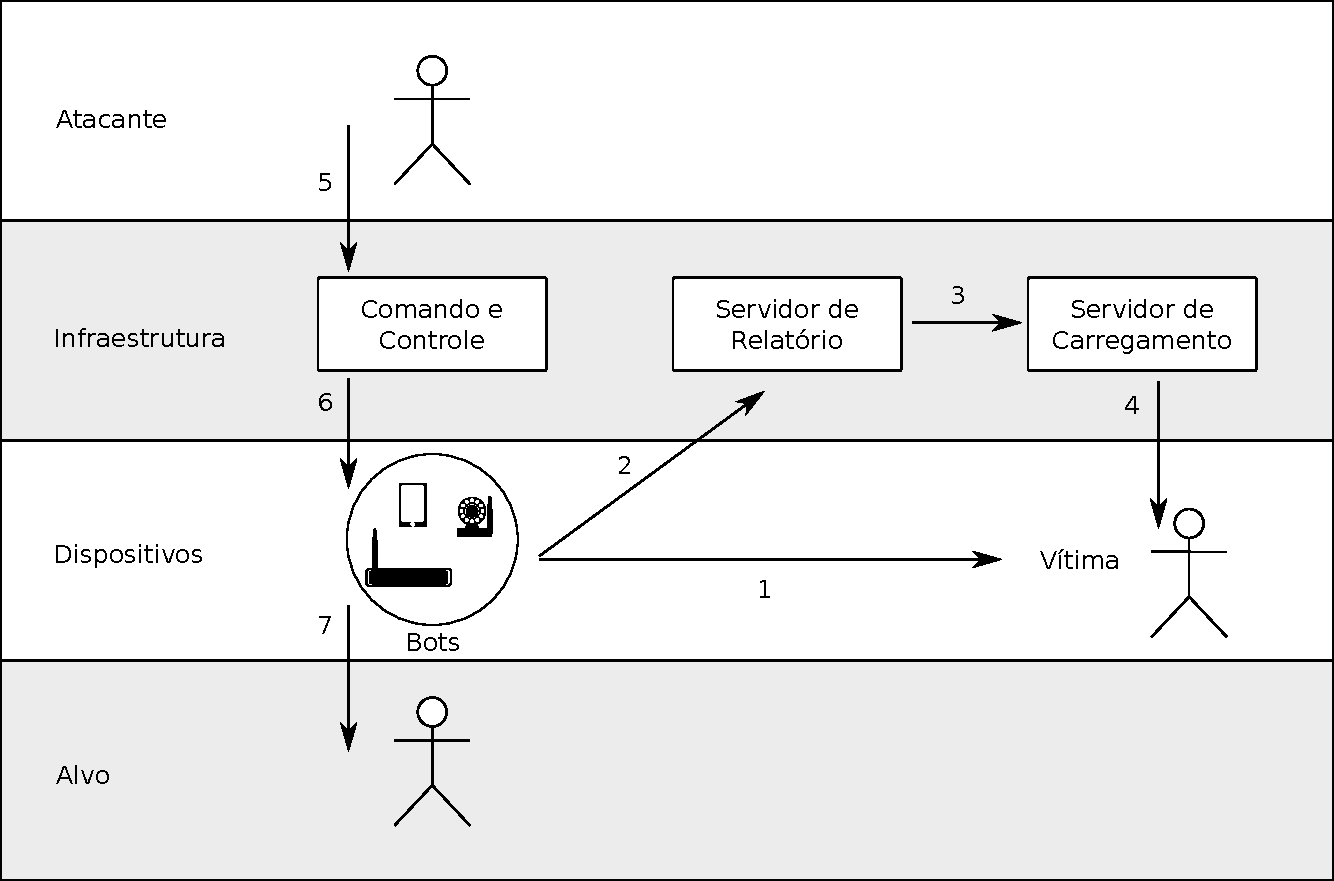
\includegraphics[width=0.7\columnwidth]{img/mirai_structure.pdf}
            \caption{Operação do Mirai.} 
            \label{fig:mirai_structure}
        \end{figure}

 
\emph{Os nossos modelos  analíticos e de  simulação focam nas contaminações dos dispositivos, ou seja, na fase de varredura (envolvendo infecções  endógenas e exógenas). Em particular, assumimos que a varredura de endereços  IPv4 pseudo-aleatórios consome recursos de banda, e que por isso a taxa de contaminações exógenas é limitada pelo \emph{poder do atacante} em função do modelo de adversário. }
    
    \textbf{Modelo de adversário}
    %    \sadoc{falar sobre adversário}
     O  adversário é o usuário que tem controle sobre o \textit{malware}. O adversário tem capacidade de reconhecer, após análise, se determinado sistema é  vulnerável, mas não é capaz de distinguir, de antemão, se determinado sistema  está, ou não, contaminado.
    Consideramos que o adversário tem uma capacidade média de contaminação exógena  de  $\Lambda$ contaminações por unidade de tempo. Essa capacidade está limitada pela taxa agregada de varredura e análise de IPs de todos os  nós que compõem a \emph{botnet}. Seja $N$ o número de nós vulneráveis na rede (ou seja, $N$ é  o número de nós que decidem não se vacinar). \emph{ No caso mais simples, supomos que a capacidade de contaminação exógena do adversário é dividida pelos nós vulneráveis presentes na rede, e que cada um é alvo de uma varredura exógena a uma taxa de  $\Lambda/N$ tentativas de contaminação por unidade de tempo.}
	
        
 
% ---------------------------------------------------------
% Evidências no mundo real

% ---
% Evidência no mundo real
% ---
\chapter{Evidências dos comportamentos seguir ou evitar a multidão }
\label{cap:evidencias}
% ---


	%%% PT-BR version
	A seguir,  visamos identificar na Internet comportamentos que se assemelhem a padrões do tipo   \textit{seguir} ou \textit{evitar} a multidão.
Para tal,	usamos dados reportados em \cite{wang2017characterizing} sobre a aplicação de \emph{patches} por parte dos usuários.    
	De acordo com \cite{wang2017characterizing}, em uma análise de mais de 64 mil amostras de dispositivos  de sistemas de controle industrial, menos de 30\% desses sistemas são atualizados para versões imunes a ataques, dentro de um prazo de 60 dias desde a descoberta da vulnerabilidade.   
	
		
%%% PT-BR version
	\section{Seleção dos dados}
	Adotamos os seguintes critérios para selecionar os sistemas cujos dados são  relevantes para nossas análises: $1)$ selecionamos sistemas que possuem pelo menos duas versões amostradas; $2)$ dado que os sistemas podem ter várias versões, para cada sistema escolhemos as versões mais populares, ou seja, as que estavam presentes em mais dispositivos durante o  histórico de medições; $3)$  excluímos os sistemas que não tiveram ao menos dez dispositivos ativos em uma única medição em qualquer uma das versões mais populares; $4)$ para facilitar e padronizar a caracterização dos sistemas selecionados, numeramos sequencialmente o número das versões, de modo que os valores menores são os mais antigos e valores maiores correspondem aos mais modernos.
	
	\section{Caracterizando o comportamento} Os típicos comportamentos de \textit{seguir} ou \textit{evitar} a multidão foram caracterizados conforme a adoção de versões mais modernas ou mais antigas. O comportamento de \textit{seguir} (resp., \textit{evitar}) a multidão ocorre quando o pico de usuários da versão mais moderna (resp., mais antiga)  \textbf{ocorre após} do pico de usuários da versão mais antiga (resp., mais moderna), mostrando que há um típico comportamento para atualizar (resp., ignorar) as versões mais recentes do sistema, que se propaga pela população.

	
	A Tabela~\ref{tab:shodam} apresenta o resultado da observação do comportamento de \textit{seguir} a multidão (S), \textit{evitar} a multidão (N) e um comportamento indefinido (I), onde não podemos caracterizar nenhum comportamento típico. As duas primeiras colunas se referem respectivamente ao índice da versão mais popular (1\textordmasculine pop) e ao dia no  qual ocorreu a  medição com  maior número de sistemas utilizando a respectiva versão (topo 1\textordmasculine) \footnote{Os dias são medidos com relação à data da primeira coleta.} e as duas próximas colunas referem-se a segunda versão mais popular. A coluna intitulada S/E/I  indica o comportamento típico da população. Para fazer a  classificação do comportamento, definimos  o índice $\iota$=(topo 1\textordmasculine - topo 2\textordmasculine) / (topo 1\textordmasculine + topo 2\textordmasculine).   O caso  $\iota > 0,01$ (resp., $\iota < -0.01$) corresponde ao comportamento de \textit{seguir} (resp., \emph{evitar})  a multidão.   Valores entre $-0,01$ e $0,01$ são  associados a comportamentos indefinidos.
	

	\begin{table}[!htb]
	    \setlength\tabcolsep{1.5pt}
		\centering
		
		\begin{tabular}{|c|c|c|c|c|l|}
			\hline
			\hspace*{-0.15cm} 1\textordmasculine pop 	 & \hspace*{-0.15cm} topo 1\textordmasculine 	 & \hspace*{-0.15cm} 2\textordmasculine pop 	 & \hspace*{-0.15cm} topo 2\textordmasculine 	 & \hspace*{-0.15cm}S/E/I& \hspace*{-0.15cm} Nome do sistema (arquivo) \\
			\hline
			\hspace*{-0.15cm} 11	& \hspace*{-0.15cm} 847	& \hspace*{-0.15cm} 6	& \hspace*{-0.15cm} 268	& \hspace*{-0.15cm} S	& \hspace*{-0.15cm} Allegro RomPager	 \\
			\hspace*{-0.15cm} 2	& \hspace*{-0.15cm} 857	& \hspace*{-0.15cm} 1	& \hspace*{-0.15cm} 854	& \hspace*{-0.15cm} I	& \hspace*{-0.15cm} AMX NetLinx A	 \\
			\hspace*{-0.15cm} 35	& \hspace*{-0.15cm} 833	& \hspace*{-0.15cm} 23	& \hspace*{-0.15cm} 850	& \hspace*{-0.15cm} E	& \hspace*{-0.15cm} Apache httpd	 \\
			\hspace*{-0.15cm} 25	& \hspace*{-0.15cm} 450	& \hspace*{-0.15cm} 21	& \hspace*{-0.15cm} 191	& \hspace*{-0.15cm} S	& \hspace*{-0.15cm} AVM FRITZ!Box Fon WLAN 7170 SIP	 \\
			\hspace*{-0.15cm} 5	& \hspace*{-0.15cm} 831	& \hspace*{-0.15cm} 2	& \hspace*{-0.15cm} 847	& \hspace*{-0.15cm} I	& \hspace*{-0.15cm} Boa HTTPd	 \\
			\hspace*{-0.15cm} 11	& \hspace*{-0.15cm} 156	& \hspace*{-0.15cm} 4	& \hspace*{-0.15cm} 857	& \hspace*{-0.15cm} E	& \hspace*{-0.15cm} Dropbear sshd	 \\
			\hspace*{-0.15cm} 6	& \hspace*{-0.15cm} 757	& \hspace*{-0.15cm} 4	& \hspace*{-0.15cm} 755	& \hspace*{-0.15cm} I	& \hspace*{-0.15cm} Lantronix MSS100 serial interface fingerd	 \\
			\hspace*{-0.15cm} 13	& \hspace*{-0.15cm} 448	& \hspace*{-0.15cm} 8	& \hspace*{-0.15cm} 311	& \hspace*{-0.15cm} S	& \hspace*{-0.15cm} lighttpd	 \\
			\hspace*{-0.15cm} 7	& \hspace*{-0.15cm} 849	& \hspace*{-0.15cm} 5	& \hspace*{-0.15cm} 848	& \hspace*{-0.15cm} I	& \hspace*{-0.15cm} Microsoft IIS httpd	 \\
			\hspace*{-0.15cm} 12	& \hspace*{-0.15cm} 850	& \hspace*{-0.15cm} 6	& \hspace*{-0.15cm} 833	& \hspace*{-0.15cm} S	& \hspace*{-0.15cm} Microsoft SQL Server	 \\
			\hspace*{-0.15cm} 2	& \hspace*{-0.15cm} 558	& \hspace*{-0.15cm} 1	& \hspace*{-0.15cm} 567	& \hspace*{-0.15cm} I	& \hspace*{-0.15cm} MoxaHttp	 \\
			\hspace*{-0.15cm} 45	& \hspace*{-0.15cm} 852	& \hspace*{-0.15cm} 36	& \hspace*{-0.15cm} 833	& \hspace*{-0.15cm} S	& \hspace*{-0.15cm} MySQL	 \\
			\hspace*{-0.15cm} 36	& \hspace*{-0.15cm} 837	& \hspace*{-0.15cm} 8	& \hspace*{-0.15cm} 848	& \hspace*{-0.15cm} I	& \hspace*{-0.15cm} nginx	 \\
			\hspace*{-0.15cm} 33	& \hspace*{-0.15cm} 852	& \hspace*{-0.15cm} 28	& \hspace*{-0.15cm} 852	& \hspace*{-0.15cm} I	& \hspace*{-0.15cm} OpenSSH	 \\
			\hspace*{-0.15cm} 17	& \hspace*{-0.15cm} 857	& \hspace*{-0.15cm} 6	& \hspace*{-0.15cm} 164	& \hspace*{-0.15cm} S	& \hspace*{-0.15cm} ProFTPD	 \\
			\hspace*{-0.15cm} 7	& \hspace*{-0.15cm} 513	& \hspace*{-0.15cm} 5	& \hspace*{-0.15cm} 521	& \hspace*{-0.15cm} I	& \hspace*{-0.15cm} Schneider BMX NOE 0100	 \\
			\hspace*{-0.15cm} 5	& \hspace*{-0.15cm} 532	& \hspace*{-0.15cm} 2	& \hspace*{-0.15cm} 525	& \hspace*{-0.15cm} I	& \hspace*{-0.15cm} Schneider BMX P34 2020	 \\
			\hspace*{-0.15cm} 8	& \hspace*{-0.15cm} 533	& \hspace*{-0.15cm} 7	& \hspace*{-0.15cm} 533	& \hspace*{-0.15cm} I	& \hspace*{-0.15cm} Schneider Electric SAS TSXETY4103	 \\
			\hspace*{-0.15cm} 8	& \hspace*{-0.15cm} 569	& \hspace*{-0.15cm} 6	& \hspace*{-0.15cm} 572	& \hspace*{-0.15cm} I	& \hspace*{-0.15cm} Siemens BACnet Field Panel	 \\
			\hspace*{-0.15cm} 3	& \hspace*{-0.15cm} 564	& \hspace*{-0.15cm} 1	& \hspace*{-0.15cm} 547	& \hspace*{-0.15cm} S	& \hspace*{-0.15cm} Siemens PXG3	 \\
			\hspace*{-0.15cm} 9	& \hspace*{-0.15cm} 1105	& \hspace*{-0.15cm} 8	& \hspace*{-0.15cm} 1096	& \hspace*{-0.15cm} I	& \hspace*{-0.15cm} Siemens SIMATIC IM151	 \\
			\hspace*{-0.15cm} 5	& \hspace*{-0.15cm} 1119	& \hspace*{-0.15cm} 4	& \hspace*{-0.15cm} 1117	& \hspace*{-0.15cm} I	& \hspace*{-0.15cm} Siemens SIMATIC S7 1200	 \\
			\hspace*{-0.15cm} 39	& \hspace*{-0.15cm} 2097	& \hspace*{-0.15cm} 38	& \hspace*{-0.15cm} 2097	& \hspace*{-0.15cm} I	& \hspace*{-0.15cm} Siemens SIMATIC S7 300	 \\
			\hspace*{-0.15cm} 18	& \hspace*{-0.15cm} 838	& \hspace*{-0.15cm} 1	& \hspace*{-0.15cm} 840	& \hspace*{-0.15cm} I	& \hspace*{-0.15cm} Tridium Niagara httpd	 \\
			\hspace*{-0.15cm} 4	& \hspace*{-0.15cm} 845	& \hspace*{-0.15cm} 3	& \hspace*{-0.15cm} 847	& \hspace*{-0.15cm} I	& \hspace*{-0.15cm} Virata-EmWeb	 \\
			\hspace*{-0.15cm} 5	& \hspace*{-0.15cm} 841	& \hspace*{-0.15cm} 4	& \hspace*{-0.15cm} 839	& \hspace*{-0.15cm} I	& \hspace*{-0.15cm} vxTarget ftpd	 \\
			\hspace*{-0.15cm} 7	& \hspace*{-0.15cm} 858	& \hspace*{-0.15cm} 5	& \hspace*{-0.15cm} 858	& \hspace*{-0.15cm} I	& \hspace*{-0.15cm} VxWorks ftpd	 \\
			\hspace*{-0.15cm} 4	& \hspace*{-0.15cm} 856	& \hspace*{-0.15cm} 3	& \hspace*{-0.15cm} 845	& \hspace*{-0.15cm} I	& \hspace*{-0.15cm} WindWeb	 \\
		\hline 	
		\end{tabular}
		\caption{Comportamento   \textit{seguir} ou \textit{evitar} a multidão, observado em populações de usuários de sistemas reais de controle industrial conectados à Internet. A maioria dos produtos possui comportamento típico de \textit{seguir} a multidão, o que vai ao encontro de \textit{evitar} a multidão, típico de sistemas biológicos.}
		\label{tab:shodam}
	\end{table}	

	A Figura~\ref{fig:shodam_example}  ilustra o número de dispositivos adotando cada uma das versões de um determinado produto, ao longo do tempo, para dois produtos distintos (Allegro RomPage e Dropbear sshd). A população do   {Allegro RomPage} possui  comportamento típico de \emph{seguir} a multidão (a versão mais nova substitui a versão mais antiga).  Já o  Dropbear sshd possui  população com comportamento  compatível com \emph{evitar} a multidão. O número de dispositivos com versão antiga cresce em conjunto com o número de dispositivos adotando a versão mais nova do produto. Este último comportamento deve-se, por exemplo, a novas instalações do produto, que muitas vezes podem vir embarcados com versões antigas do firmware.  Mesmo que o comportamento de \emph{evitar} a multidão não esteja sendo tomado de forma consciente e estratégica, os seus impactos são os mesmos que aqueles observados numa população em que indivíduos param de aplicar uma vacina (contramedida), por considerar que a ameaça é desprezível.  Eventualmente,  a população pode  se ver em face a uma epidemia de um vírus que se pensava erradicado.  


	\begin{figure}[!htb]
	%	\centering
	\hspace{-0.2in}	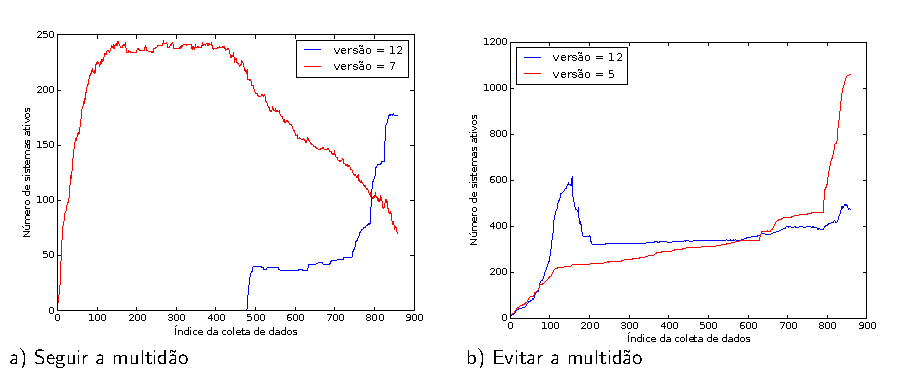
\includegraphics[width=1.0\columnwidth,keepaspectratio=false]{./img/shodam_example.pdf}
		\caption{a) Comportamento de seguir a multidão : sistema Allegro RomPage. b)Comportamento de evitar a multidão: sistema  Dropbear sshd}
		\label{fig:shodam_example}
	\end{figure}

		
% ---------------------------------------------------------
% Modelo Epidemico

% ---
% Modelo Epidemiológico
% ---
\chapter{Modelo Epidêmico}
\label{cap:modelo_epidemico}
% ---
    A seguir, analisamos o modelo epidemiológico SIS multiplicativo, conforme apresentado em \cite{rufino2018contaminaccao}.  As Seções~\ref{sec:descrmodel} e~\ref{sec:modelbinon} descrevem o  modelo.  
    A Seção~\ref{sec:otimon} apresenta resultados sobre o estado mais provável, seguida pela  busca dos valores ótimos para parametrizar o modelo, relacionando tais valores com o estado mais provável.

	\begin{table}[!htb]
	\footnotesize
		\centering 
			\caption{Tabela de notação}
		\begin{tabular}{clc}
			\hline
			variável 		& descrição 								& valor de referência \\ 
			\hline
			$M$ 			& tamanho total da população 				& 100 \\
			$N$ 			& população passível de infecção 			& M\\
			$\gamma$ 		&  fator de infecção endógena (por aresta) 	& 1.09 \\
			$\lambda$ 		&  fator de infecção exógena (por nó) 		& $\Lambda/N$ \\ 
			$\Lambda$ 		& fator de infecção exógena total 			& 10 \\
			$A$ 			& matriz de adjacência (conexões) 			& completa \\
			$d$ 			& número de nós vizinhos infectados 		& - \\
			$\lambda \gamma^d$ &  taxa de infecção (por nó)  			& - \\
			$\mu$ 			& taxa de recuperação 						& 1 \\
			$\pi(\bm{x})$ 	& probabilidade do estado $\bm{x} $			& - \\
			$i$  			& número de nós infectados na rede 			& - \\
			$\rho$ 			& probabilidade de um nó escolhido ao acaso estar contaminado & - \\
			\hline
		\end{tabular}
 	\label{tab:notation}
	\end{table}
	
    \section{Descrição do modelo}  
    \label{sec:descrmodel}
    	Consideramos uma população finita contendo $M$ nós, dos quais, $N$ decidiram não vacinar, e portanto possuem uma vulnerabilidade que pode ser explorada.	Cada um desses $N$ nós pode assumir os estados de suscetível ($S$ ou $0$) ou infectado ($I$ ou $1$). 
    	
    	Um nó infectado pode ser recuperado, passando do estado $I$  para o estado $S$ após um tempo  exponencialmente distribuído com média 
    	$1/\mu$.
    	Um nó suscetível pode ser infectado por um atacante externo (infecção exógena) ou por um ataque interno (infecção endógena) de um vizinho na rede. Seja $d$ o número de vizinhos infectados.  
    	Seja $\gamma$ a taxa de infecção endógena por vizinho e seja $\lambda$ a taxa de infecção exógena por nó, $\lambda = \Lambda /N$.  
    	Assumimos que o tempo entre  infecções é exponencialmente distribuído, com taxa  $\gamma^d \lambda$. Ou seja, assumimos contribuições  multiplicativas das taxas de infecções endógenas e exógenas.  

    	Seja $\bx$ um estado possível da rede, entre todos os estados possíveis $\mathcal{X}$. O estado é um vetor $N$ dimensional, $\bx \in \{0,1\}^N$, $\bx=(x_1, x_2, \cdots, x_k, \cdots, x_{N-1},x_{N})$, onde $x_k \in \{0,1\}$. A dinâmica do sistema é caracterizada por um processo Markoviano contínuo, homogêneo temporal, irredutível e de estados finitos. Cada estado da rede corresponde a um estado no processo Markoviano. Além disso, o nosso processo Markoviano é reversível, conforme \cite{kelly1979reversibility}.

    	Consideramos uma topologia totalmente conectada, onde todos os nós estão conectados entre si. A probabilidade do estado $\bx$ é dada por $\pi(\bx)$, derivada em~\cite{zhang2017contact},
    	\begin{eqnarray}
    	    \pi(\bx) & = & \frac{\tilde{\pi}(\bx)}{Z} \label{eq:equilibriumBasicScaledSIS}
    	\end{eqnarray}
	    onde
        \begin{equation}
            \tilde{\pi}(\bx)=\left( \frac{\lambda}{\mu}\right)^{1^{T}\bx} \gamma^{\bx^{T}A\bx/2} \textrm{ , } \bx \in \mathcal{X}, \qquad 	  Z= \sum_{\bx \in \mathcal{X}} \tilde{\pi}(\bx). \label{eq:equilibriumNumeratorScaledSIS}
        \end{equation}
        A Tabela~\ref{tab:notation} resume a notação.  

        Tomando proveito da simetria do problema, e com certo abuso de notação, seja $\pi(\iota)$ a probabilidade de haver $\iota$ nós infectados:
        \begin{equation}
            \pi(\iota) = \frac{\tilde{\pi}(\iota)}{Z}, \qquad \tilde{\pi}(\iota) = \binom{N}{\iota} \left(\frac{\lambda(N)}{\mu}\right)^{\iota} \gamma^{\iota(\iota-1)/2}, \quad \iota=0, \ldots, N.  \label{eq:scaledSISProbIotaInfected}
        \end{equation}

	    O valor esperado do número de nós infectados é
    	\begin{equation}
    	    E(I) = \sum\limits_{\iota = 0}^{N} \iota \frac{\tilde{\pi}(\iota)} {Z} = N\rho(N), \quad \rho(N) = \frac{1}{N} \sum\limits_{\iota = 0}^{N} \iota \frac{\tilde{\pi}(\iota)}{Z} \label{eq:scaledSIS_espected_infecteds}
    	\end{equation}
	    onde $\rho(N)$	é a probabilidade de  infecção de um nó escolhido aleatoriamente. 

    \section{Aproximação binomial} \label{sec:modelbinon}
	    A análise direta das equações acima é complexa, por envolver um termo quadrático no expoente de $\gamma$ em \eqref{eq:scaledSISProbIotaInfected}.  Para simplificar a análise, consideramos  uma solução aproximada. Para tal, definimos $\hat\rho(N) \approx \rho(N)$ e $\hat\pi(\iota) \approx \tilde\pi(\iota)$:
		\begin{align}
		  \hat {\rho}(N)	&=  \frac{1}{N} \sum\limits_{\iota=0}^{N}\iota \frac{\hat{\pi}(\iota)}{{\hat Z}}, \quad \hat{Z} = \sum\limits_{\iota=0}^{N} \hat{\pi}(\iota), \quad \hat{\pi}(\iota)	=  \binom{N}{\iota} \left(\frac{\lambda(N)}{\mu}\gamma^{N^{\star}}\right)^{\iota}\label{eq:rho_Nhat1} 
		\end{align}
		onde $N^{\star}(N)$ é uma função crescente de $N$, que denotamos simplesmente por $N^{\star}$ para simplificar a notação.  Nos referimos ao modelo proposto para aproximar a solução do modelo original como \emph{modelo binomial}, por fazermos uso do binômio de Newton na demonstração do resultado a seguir. 

		\begin{lemma}
			No modelo binomial,  temos que:
				\begin{equation}
							\hat{\rho}(N) =   \frac{1}  {1+ \mu/(\lambda(N) \gamma^{N^{\star}} )  }  \label{eq:mainlema} %\tag{3} \label{e}
				\end{equation} 
		\end{lemma}	

		A demonstração do lema acima consta em  \cite{rufino2018contaminaccao}, notando o pequeno ajuste de notação na nova versão do resultado, refletindo a nova definição de $N^{\star}$.

	    Como discutido na Seção~\ref{sec:otimon} a seguir, $N^{\star}$ é adequadamente parametrizado como $N^{\star} = (N-1)\hat{\rho}(N)$. Simplificando a notação,  removendo as dependências  com relação a $N$,

		\begin{equation}
			\hat{\rho} =   \frac{1}  {1+ \mu/(\lambda \gamma^{(N-1)\hat{\rho}} )  }  \label{eq:mainlema1} %\tag{3} \label{e}
		\end{equation} 
	    A equação acima dá origem a um problema de ponto fixo, analisado na Seção~\ref{sec:fechada}.

        \begin{figure}[!htb]
    		\centering
    	    \hspace{-0.2in}	
            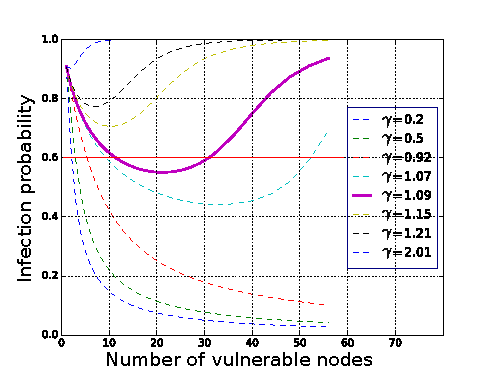
\includegraphics[width=0.49\columnwidth,keepaspectratio=true]{./img/scaled_sis_lambda_10_EN_curves.pdf}
    		\caption{Equilíbrio em relação as motivações para vacinar ou não vacinar ($\gamma=1,09$).}
    		\label{fig:equilibrim_cost}
        \end{figure}


	\section{Buscando valor ótimo para  \texorpdfstring{$N^{\star}$}{N*}}
	\label{sec:otimon}
		A seguir, buscamos o valor ótimo de $N^{\star}$ em função de $N$.  Para tal, nos aproveitamos de um resultado recentemente derivado em~\cite{zhang2018more} sobre os estados mais prováveis do modelo epidemiológico  aqui discutido. Em~\cite{zhang2018more}, os autores discutem o cenário no qual  a taxa de infecção exógena, $\lambda$, é constante, independente de $N$.   Reproduzimos o principal resultado de~\cite{zhang2018more}, tendo em vista que ele  nos traz \emph{insights} sobre o valor ótimo de $N^{\star}$. 

		Seja $\bx^{\star}$ a \textit{configuração mais provável} do sistema,  $\bx^{\star} = [x_1^{\star}, x_2^{\star}, \ldots, x_{N}^{\star}]$, onde $\bx^{\star} = \argmax\limits_{\bx \in \mathcal{X}} \: \pi(\bx)$. 
		Se $\tilde{\pi}(\bx^{\star}) \gg \tilde{\pi}(\bx)$ , $\forall \bx \in \mathcal{X}\slash \bx^{\star}$, então 
        \begin{equation}
        	P(x_{k} =1) \approx  \frac{1}{1+\mu/\left(\lambda\gamma^{m_{k}^{\star}}\right)}, \quad \textrm{, onde }  m_{k}^{\star}=\sum\limits_{j=1}^{N} a_{kj}x_{j}^{\star}. \label{eq:aproximacao_Zhang}
        \end{equation}
		O resultado acima decorre do fato de que a probabilidade do estado $\bx$ pode ser expressa como $\pi(\bx)=e^{H(\bx)}$, onde $H(\bx)=1^{T} \bx \: \log \left( {\lambda}/{\mu} \right) + \left( \bx^{T} A \bx \: \log \gamma\right) /2$.  Notando então a  relação entre $\pi(\bx)$ e a distribuição de Gibbs, o resultado segue.
        
		Note que  $m_{k}^{\star}$ representa o números de vizinhos de $k$  contaminados no estado mais provável. Comparando~\eqref{eq:aproximacao_Zhang} e~\eqref{eq:mainlema}, vemos que $m_{k}^{\star}$ está  diretamente relacionado a $N^{\star}$.  
		Seja $n$ o número de vizinhos de um nó típico.  Ao considerarmos um  grafo completo, o número de vizinhos de cada nó é $n=N-1$, e o número médio de vizinhos contaminados é $\rho n$.  Substituindo $N^{\star}$ em~\eqref{eq:mainlema} por $m_k^{\star}$,  obtemos então a expressão~\eqref{eq:aproximacao_Zhang}.
		Tal argumento sugere que o valor ótimo de $N^{\star}$ é dado por $N^{\star}=\hat{\rho}  n$.   A seguir, ilustramos numericamente tal fato.

		A Figura~\ref{fig:result_01b} ilustra como  a probabilidade de infecção  em função do número de nós não vacinados na rede, $N$. Consideramos $\lambda=\Lambda/N$, $\Lambda=10$, $\mu=1$ e $\gamma=1.09$.   O valor de $\hat{\rho}$ obtido via aproximação, quando selecionamos o melhor valor de $N^{\star}$, é muito próximo do valor de $\rho$ exato.  A Figura~\ref{fig:result_01b}(a) mostra também que quando fazemos $N^{\star}=N$ e $N^{\star}=N/2$ obtemos limites superiores e inferiores para a probabilidade de contaminação. Para avaliar a qualidade da aproximação $N^{\star}=\rho (N-1)$, a Figura~\ref{fig:result_01b}(b) mostra o valor ótimo de $N^{\star}$, em função de $N$, comparado com $N/2$, $\rho N$ e $\rho (N-1)$. Tanto $\rho N$ quanto $\rho (N-1)$ apresentam excelentes aproximações.  Calculando a soma dos erros quadráticos (em destaque na figura), podemos identificar que de fato $\rho(N-1)$ é uma melhor aproximação, corroborando os resultados derivados nessa seção. 
		

    \section{Fórmulas fechadas via método de Newton}
    \label{sec:fechadageral}
    	A seguir indicamos como usar o método de Newton para achar fórmulas fechadas aproximadas para~\eqref{eq:mainlema}.
	    Pelo fato de $\rho$ aparecer tanto do lado direito quanto do lado esquerdo de~\eqref{eq:mainlema}, a equação não é passível de solução exata em fórmula fechada.  Ao invés de buscar por soluções exatas, buscamos então por aproximações. Para tal, vamos considerar as seguintes funções auxiliares, 
    	\begin{eqnarray}
    		f(\rho)		&=& 	\rho \left( 1 + \frac{\mu}{\lambda}\gamma^{-\rho n} \right) -1  =  
    							\rho + \rho \frac{\mu}{\lambda} \gamma^{-\rho n} -1 \label{eq:2} \\
    		\frac{ \partial{f(\rho)}}{ \partial \rho}  = 
    		f'(\rho)	&= &	1 + \frac{\mu}{\lambda} \gamma^{-\rho n} 
    							\left( 1 - \rho n \ln \gamma \right)  \label{eq:3} \\
    		\frac{\partial^2{f(\rho)}}{ \partial^2 \rho}  = 
    		f''(\rho)	&= & 	g \frac{\mu \ln \gamma}{\lambda} \gamma^{-\rho n} 
    							\left( \rho (\ln \gamma) -2 \right)  \label{eq:4}
    	\end{eqnarray}
    	Encontrar a solução $\rho$ para~\eqref{eq:mainlema1} é equivalente a encontrar as raízes (i.e., os zeros) de~\eqref{eq:2}.

	    A iteração  do método de Newton, adaptada ao nosso cenário, é dada por,
	    \begin{equation}
	        \rho_{i+1} =  \rho_{i} - \frac{f(\rho_{i})}{f'(\rho_{i})} = \frac{\lambda-\mu\gamma^{-\rho_{i}n} \left(\rho_{i}^{2} n\ln\gamma\right)}{\lambda-\mu \gamma^{-\rho_{i}n} \left(\rho_{i}n \ln\gamma-1\right)} \label{eq:newton_general}
	    \end{equation}
	    Destacamos que $f(0)=-1$ e $f(1) = \frac{\mu}{\lambda \gamma} > 0$, onde $ \mu, \lambda > 0$ e $\gamma > 1$.  Além disso, $f(0)=-1$ e $ f'(0) =  {\mu}/({\lambda \gamma})$, assim como $ f''(0) = {\mu \ln \gamma}/{\lambda}$.  Desta forma, se $\gamma > 1$, então $f(0)  f''(0) > 0$ ($f$ e $f''$ têm o mesmo sinal). Pelo teorema  de  Darboux \cite{mikusinski1955methode}, iniciando com  $\rho_0 = 0$, o método de Newton converge sem  ultrapassar (\emph{overshoot}) a solução.


	\section{Obtendo fórmulas fechadas}
	\label{sec:fechada}
		Usando a abordagem descrita acima, obtemos  fórmulas fechadas para uma aproximação da probabilidade de um nó estar infectado.  Numericamente, identificamos que considerar  duas iterações do método de Newton é suficiente para obter boas aproximações.

		A condição inicial do método de Newton tem um papel importante no resultado.  Consideramos então duas condições iniciais extremas. Seja $\rho_0$ a condição inicial do método.  Considerando $\rho_0=0$ e $\rho_0=1$, obtemos duas aproximações para a probabilidade de contaminação.  Na próxima seção, apresentamos uma heurística simples para determinar quando adotar uma condição inicial ou a outra.  Na Seção~\ref{sec:fechadageral}, indicamos numericamente que as aproximações junto com a heurística capturam o comportamento da probabilidade de infecção.

		Seja $\rho_i^{(0)}$ a probabilidade de infecção aproximada após $i$ iterações do método de Newton, com condição inicial $\rho_0=0$. Então, 
			 \begin{eqnarray}
			  \rho_{0}^{(0)} &=& 0, \quad \rho_1^{(0)} = \frac{\lambda}{\lambda + \mu}   \nonumber \\
			  \rho_{2}^{(0)} &=& \frac{ \lambda - \mu \gamma^{-\rho_{1} n }  \left( \rho_{1}^{2} n  \ln \gamma    \right) }  
		                            { \lambda - \mu \gamma^{-\rho_{1} n }  \left( \rho_{1}     n  \ln \gamma  -1 \right) } \nonumber =  \frac{ \lambda - \mu \gamma^{-\left( \frac{\lambda}{\lambda + \mu} \right) n }  \left( \left( \frac{\lambda}{\lambda + \mu} \right)^{2} n  \ln \gamma    \right) }  
		                            { \lambda - \mu \gamma^{-\left( \frac{\lambda}{\lambda + \mu} \right) n }  \left( \left( \frac{\lambda}{\lambda + \mu} \right)     n  \ln \gamma  -1 \right) } \label{eq:rho_2iter_rho0_0}
			 \end{eqnarray}

		Analogamente, seja $\rho_i^{(1)}$ a probabilidade de infecção aproximada após $i$ iterações do método de Newton, com condição inicial $\rho_0=1$. Então, 
 
    	\begin{equation}
    	  \rho_2^{(1)}    = \frac{ \lambda - \mu \gamma^{-\left( \frac{ \lambda - \mu \gamma^{- n }  \left( n  \ln \gamma    \right) }  { \lambda - \mu \gamma^{- n }  \left( n  \ln \gamma  -1 \right) }  \right) n } \left( \left( \frac{ \lambda - \mu \gamma^{- n }  \left( n  \ln \gamma    \right) }  { \lambda - \mu \gamma^{- n }  \left( n  \ln \gamma  -1 \right) }  \right)^{2} n \ln \gamma \right) }  
    		                    { \lambda - \mu \gamma^{-\left( \frac{ \lambda - \mu \gamma^{- n }  \left( n  \ln \gamma    \right) }  { \lambda - \mu \gamma^{- n }  \left( n  \ln \gamma  -1 \right) }  \right) n } \left( \left( \frac{ \lambda - \mu \gamma^{- n }  \left( n  \ln \gamma    \right) }  { \lambda - \mu \gamma^{- n }  \left( n  \ln \gamma  -1 \right) }  \right)     n \ln \gamma -1 \right) } 
    		                    \label{eq:rho_2iter_rho0_1}
    	\end{equation}
	    A fórmula fechada com $\rho_0=0$ é bem mais simples que com $\rho_0=1$. Conforme iremos indicar nas seções a seguir, para muitos cenários a primeira aproximação, mais simples, é suficiente.  


    	\subsection{Heurística para determinação da condição inicial}
	    \label{subsec:heuristica}
    	A seguir consideramos uma heurística para determinar a condição inicial ótima da iteração de Newton descrita na seção anterior.  Para tal, ilustramos o comportamento da aproximação quando $\rho_0=0$ na Figura~\ref{fig:rho_exact_approx_newton_rho0_0e1}(a) e $\rho_0=1$ na Figura~\ref{fig:rho_exact_approx_newton_rho0_0e1}(b) exceto a curva para $\gamma=1.03$, usando os valores referência na Tabela~\ref{tab:notation}. % Os demais valores, quando não for explicitamente dito, usaremos os valores de referência da Tabela~\ref{tab:notation}. 
    	Na medida em que $N$ aumenta, a condição inicial $\rho_0=1$ tende a produzir melhores aproximações.  Entretanto, para valores pequenos de $\gamma$ (e.g., $\gamma=1,03$) é preciso utilizar a condição inicial $\rho_0=0$ mesmo para valores grandes de $N$.

    	\begin{figure}[!htb]
    	    \centering
    	    \begin{tabular}{cc}
    	         \hspace{-1.2cm}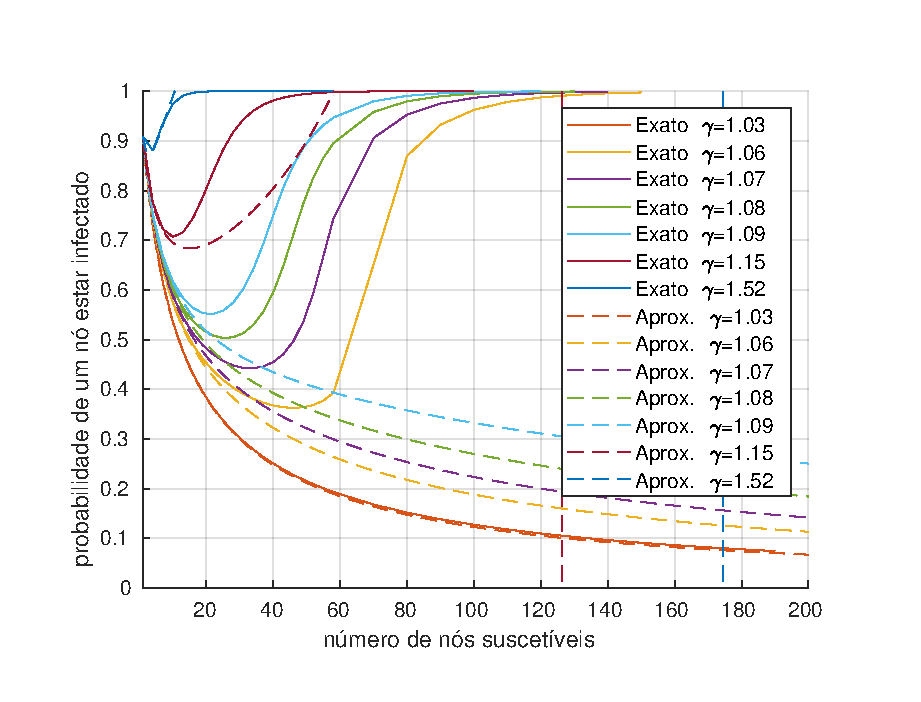
\includegraphics[width=0.6\columnwidth]{img/exact_approx_v0_lambda10_00_gamma1_52_iter_2_rho0_0.pdf}&
    	         \hspace{-1.2cm}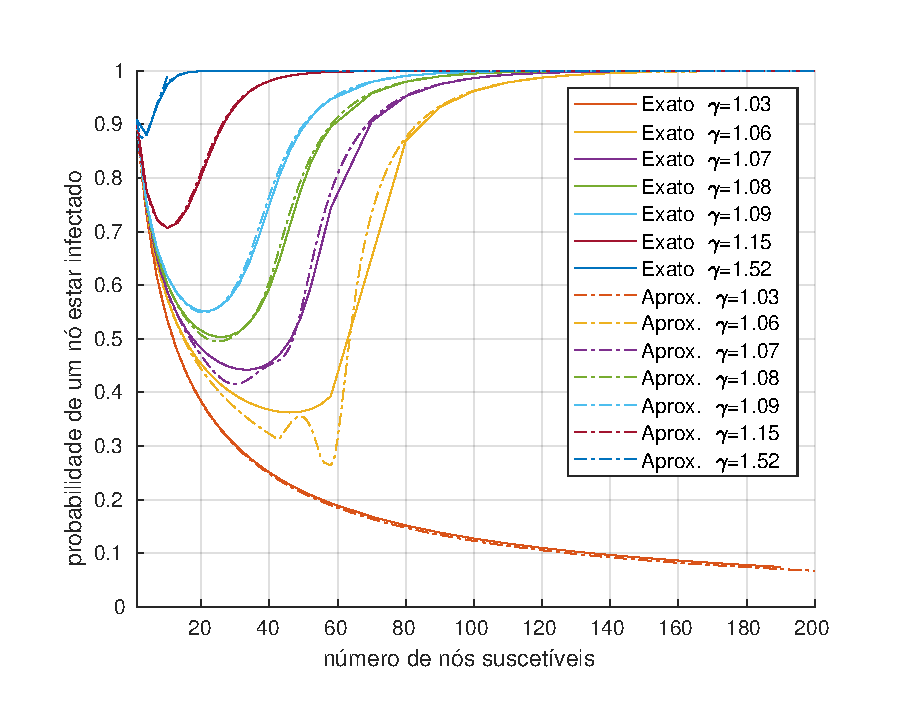
\includegraphics[width=0.6\columnwidth]{img/exact_approx_lambda10_00_gamma1_52_iter_2.pdf}\\
    	         \hspace{-1.2cm}(a) $\rho_{0}=0$ & \hspace{-1.2cm}(b) $\rho_{0}$ dado por~\eqref{eq:heuri} 
    	    \end{tabular}
    	   \caption{Probabilidade de infecção, calculada usando método de Newton com (a)  condição inicial $\rho_0=0$ e (b) heurística para condição inicial.}
    	    \label{fig:rho_exact_approx_newton_rho0_0e1}
    	\end{figure}

        Dependendo da condição inicial, o método de Newton pode  convergir para valores maiores que 1 ou menores que 0. Como ilustrado na Figura~\ref{fig:rho_exact_approx_newton_rho0_0e1}(a),  para $\gamma=1,52$ e $1,15$. Portanto, nossa  heurística para determinar  a  inicialização parte da definição das seguintes quantidades auxiliares adicionais,
        \begin{equation}
    	    \bar{\rho}_2^{(z)}(N) = \left\{
            \begin{array}{ll}
                {\rho}_2^{(z)}(N), & \textrm{se } 0 \leq {\rho}_2^{(z)}(N) \leq 1 \textrm{ e } \bar{\rho}_2^{(z)}(N-1) \neq -\infty, \\
    	        -\infty, & \textrm{caso contrário.}
            \end{array}\right. \label{eq:condi}
    	\end{equation}
	    onde $z$ é a condição inicial, $0 \leq z \leq 1$.
	    Segundo~\eqref{eq:condi}, se o método de Newton convergir para valores além do domínio de interesse para determinada condição inicial, tal condição é descartada daí em diante.  Em~\eqref{eq:condi} deixamos explícita a dependência de $\rho$ com relação a $N=n+1$ (na Seção~\ref{sec:fechada} tal dependência foi mantida implícita). Motivado pela discussão acima, nossa heurística é então dada por,
    	\begin{equation} \label{eq:heuri}
    	    \bar{\rho}(N) = \max(\bar{\rho}_2^{(0)}(N), \bar{\rho}_2^{(1)}(N))
    	\end{equation}
	    A Figura~\ref{fig:rho_exact_approx_newton_rho0_0e1}(b) ilustra a qualidade das aproximações obtidas por meio da heurística de inicialização. Para os cenários em consideração a heurística foi capaz de determinar boas escolhas para inicializar os parâmetros. 

	\section{Vacinar, reiniciar ou esperar?}
	    Tendo em vista a solução com fórmulas fechadas descrita nesta seção, podemos gerar curvas como aquela apresentada na Figura~\ref{fig:rho_exact_approx_newton_rho0_0e1} de forma bem eficiente.  Dada esta curva, assumimos então um custo fixo da contramedida mais custosa (vacinar).  Para fins de ilustração, consideramos que o custo é dado pela  probabilidade de um nó estar infectado. % Por exemplo, o custo pode refletir  a probabilidade de ocorrer uma catástrofe. 
	    A utilidade do usuário é dada então pela diferença entre a probabilidade de infecção  e o custo.   Considere, por exemplo, o caso $\gamma=1,07$ na Figura~\ref{fig:rho_exact_approx_newton_rho0_0e1} e o custo igual a $0,5$.  Segundo a Figura~\ref{fig:rho_exact_approx_newton_rho0_0e1}, se o número de nós não vacinados for menor ou igual a 20, a probabilidade de infecção é alta e os nós tem incentivos para se vacinarem (sistema dominado por infecções exógenas).  Por outro lado, se o número de nós não vacinados variar entre 20 e 50, o custo de vacinação é superior à probabilidade de infecção. Nesse caso,  os nós tem incentivo para não vacinarem-se, e simplesmente esperarem e reiniciarem suas máquinas quando detectarem um ataque (de forma reativa) ou quando avaliarem que o sistema está ocioso (de forma proativa).   

	    \textbf{Mensagem desta seção} Nesta seção, apresentamos fórmulas fechadas para estimar a probabilidade de contaminação de nós na rede.  As fórmulas fechadas podem ser usadas para guiar a tomada de decisão com relação a contramedidas (e.g., vacinar, reiniciar ou esperar, conforme discutido acima).  Na seção a seguir, indicamos por meio de simulações que de fato os regimes discutidos acima, nos quais diferentes contramedidas são adotadas, também são observados nos cenários simulados.  


% ---------------------------------------------------------
% Simulação

% ---
% Simulação
% ---
\chapter{Simulação}
\label{cap:simulacao}
% ---


% \subsection{Descrição do simulador}

    Nesta seção apresentamos o simulador de propagação de \emph{malware} construído para reproduzir o comportamento descrito no Capítulo~\ref{cap:descricao}. Nossos objetivos são $(i)$ ilustrar o comportamento do sistema sob condições diferentes do modelo analítico, e.g., assumindo que os nós podem entrar e sair da rede, e que os tempos entre eventos não são necessariamente exponenciais e $(ii)$  comparar os resultados do modelo analítico contra simulações.  Nosso simulador é flexível e permite a avaliação de \emph{malware} com diferentes padrões de comportamento, que descrevemos a seguir.

    \textbf{Configuração do simulador} 
    O simulador construído permite verificar o comportamento e dinâmica de uma rede, sob a perspectiva de um ataque de código malicioso tipo \emph{Botnet Mirai}, contando com um atacante estratégico, o \textit{Botmaster}.  As contaminações se dão pelo  processo de varredura, autenticação e infecção descrito no Capítulo~\ref{cap:descricao}.
    %, conforme o esquema da Figura~\ref{fig:esquema_mirai_bot_simulador}.  
    As tentativas de autenticação podem falhar porque o dispositivo alvo é seguro ou porque já foi infectado. Em ambos os casos, o dispositivo alvo não responde à tentativa de autenticação.

    O \textit{botMaster} busca por \emph{hosts} vulneráveis e troca mensagens para realizar a infecção.  Caso a latência seja superior a um \textit{timeout} determinado, a contaminação falha. 
    A taxa de contaminação do \textit{botMaster} é fixa, independente do número de nós na rede.  No modelo, tal taxa corresponde ao parâmetro $\Lambda$.   A taxa de contaminação exógena por \emph{host} é $\lambda=\Lambda/N$.  
    Cada \emph{host} contaminado torna-se um \textit{bot}, que pode iniciar o processo de contaminação de todos os \emph{hosts} vulneráveis alcançáveis.  Tal contaminação endógena começa por uma autenticação na vítima, seguida pelo processo de tentativa de infecção. 
    Os parâmetros do simulador com seus valores de referência estão listados na Tabela~\ref{tab:sim.params}.
    

    

\begin{comment}
Em particular, o simulador permite execução de redes com diferentes
quantidades $N$ e $M$ de dispositivos vulneráveis e seguros, i.e., que podem e não podem ser infectados pelo \emph{malware},
respectivamente.  Também é possível configurar a quantidade $N_m$ de
dispositivos que executam o \emph{malware} continuamente.  Os
dispositivos vulneráveis e seguros poder ser desligados e religados.
As durações dos períodos nos quais os dispositivos permanecem
ligados e desligados são amostradas de distribuições estatísticas,
$D_\textrm{on}$ e $D_\textrm{off}$, respectivamente.  Para capturar
a volatilidade de \emph{malwares} comuns em dispositivos IoT, que
não possuem armazenamento persistente, o simulador considera que um
dispositivo vulnerável volta à configuração de fábrica (i.e., não
infectado) quando é religado.
\end{comment}

	\begin{table}[!htb]
		\footnotesize
	\centering
		\caption{Parâmetros  do  simulador e  valores de referência.}
	\begin{tabular}{lll}
	        \textsc{Param.} & 
	        \textsc{Descrição} & 
	       \textsc{Referência}\\ 
	        \hline
	        \hline
	        \multicolumn{3}{l}{\emph{Tamanho da rede}} \\
	        $M$ & 
	        Total de indivíduos &  
	        $10$ a $500$ \\
	        \hline
	        $N_p=N/M$ & 
	        Proporção de indivíduos vulneráveis (não vacinados) 
	        & $100\%$ \\
	        \hline
	        \hline
	        \multicolumn{3}{l}{\emph{Comportamento dos dispositivos}} \\
	        $\mathcal{D}_\textrm{on}$ & 
	        Distribuição do período ligado (up-time) &
	        Exponencial \\
	        \hline
	        $P_{\mathcal{D}_{\textrm{on}}}$ & 
	        Parâmetros que definem a distribuição &
	        Média de $65$ \\
	         & 
	         do período ligado (Média, Variância, ...) & 
	         unid. tempo\\
	        \hline
	        $\mathcal{D}_\textrm{off}$ & 
	        Distribuição do período desligado  (down-time) &
	        Exponencial \\
	        \hline
	        $P_{\mathcal{D}_\textrm{off}}$ & 
	                Parâmetros que definem a distribuição &
	        Média de $0,1$ \\
	         & 
	         do período desligado (Média, Variância, ...) & 
	         unid. tempo\\
	        \hline
	        \hline
	        \multicolumn{3}{l}{\emph{Latência fim-a-fim}} \\
	        $l_\textrm{min}$ e $ l_\mathrm{max}$ & 
	        Latência fim-a-fim mínima e máxima,  & $
	        0,01$ e $0,4$ \\
	         & sendo latência uniformemente distribuída & \\
	        \hline
	        $T$ & 
	        \textit{Timeout}, tempo máximo de conexão 
	        & $2,0$ \\
	        \hline
	        $m_\textrm{auth}$ & 
	        Mensagens em uma tentativa de autenticação & 
	        $7$\\
	        \hline
	        $m_\textrm{infect}$ & 
	        Mensagens em uma tentativa de infecção & 
	        $700$ \\
	        \hline
	        \hline
	        \multicolumn{3}{l}{\emph{Comportamento do malware}} \\
	        $\mathcal{B}_\mathrm{exe}$ & 
	        Modelo de execução do \textit{bot} & ``BroadcastBot'' \\
	        \hline
	        $\beta_{\mathcal{B}_\mathrm{exe}}$ & 
	        Parâmetro do modelo de execução do \textit{bot} &
	        Taxa de contaminação\\
	        & & $5\times10^{-5}$ \\
	        \hline
	        $\mathcal{M}_\mathrm{exe}$ & 
	        Modelo de execução do \textit{botMaster} &
	        ``UnicastBot'' \\
	        \hline
	        $\alpha_{\mathcal{M}_\mathrm{exe}}$ & 
	        Parâmetro do modelo de execução do \textit{botMaster} & 
	        Taxa de contaminação\\
	        & & $2\times10^{-2}$ \\
	        \hline
	        \hline
	\end{tabular}
	\label{tab:sim.params}
	\end{table}


	\textbf{Resultados de simulação}  
	    Os  resultados da simulação estão sumarizados na Figura~\ref{fig:simulacao_resultados_1a_parte}, onde apresentamos a proporção média da população vulnerável  infectada (vermelho) e desligada (verde)  em função do números de nós vulneráveis ($N$).  Cada curva reflete a média de  oito  rodadas de simulações.  As linhas pontilhadas e tracejadas representam o número de nós infectados de forma endógena e exógena, respectivamente.  Somando os valores correspondentes a estas duas linhas, obtemos a fração de nós infecatdos (linha vermelha). 
	    

	    
	    
	\begin{figure}
	    \centering
	    \begin{tabular}{ccc}
	        \hspace{-0.6cm}Taxa de infecção endógena & 
	        \hspace{-0.6cm}Taxa de Infecção exógena & 
	        \hspace{-0.6cm}Tempo médio ligado\\
	        %------------------------------------------------------
	        \hspace{-0.6cm}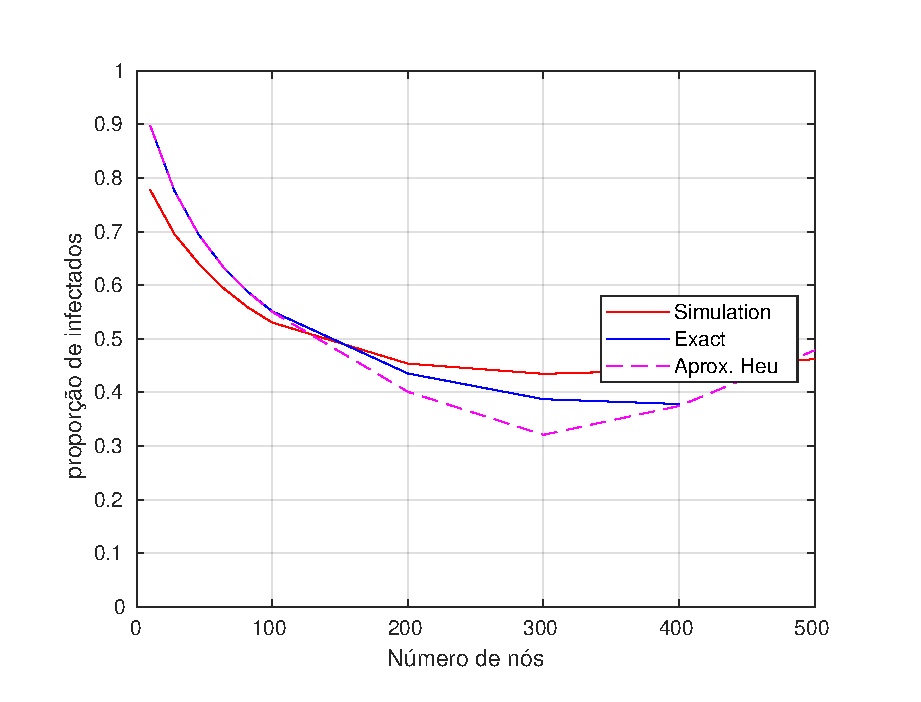
\includegraphics[width=0.35\columnwidth]{img/fig_a_1000_v0_lambda1500_mu17_9593_gamma1_007100_iter_2_rho0_0.pdf} & 
	        \hspace{-0.6cm}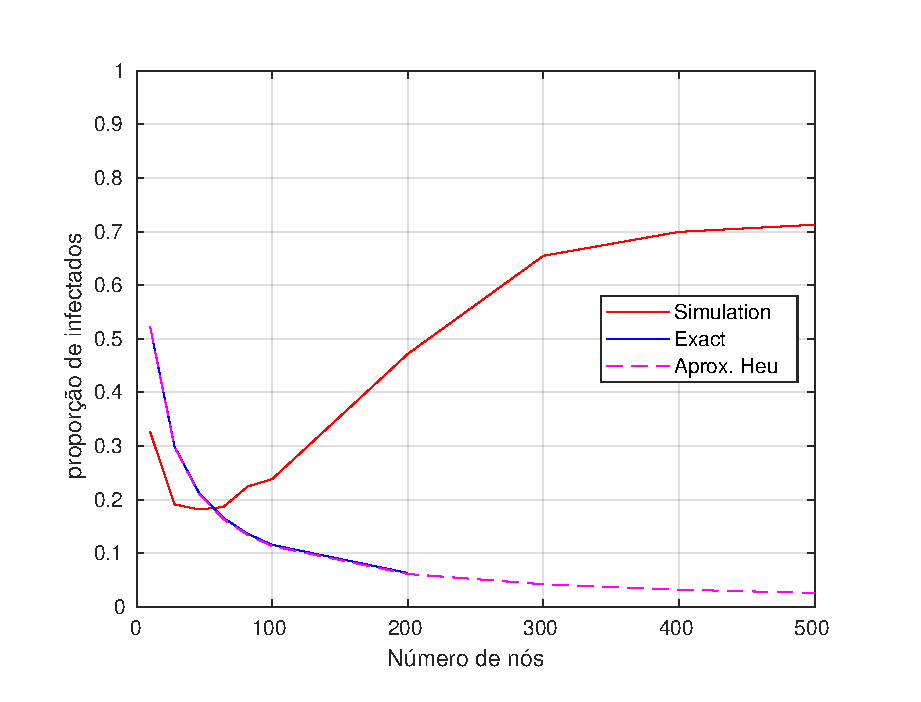
\includegraphics[width=0.35\columnwidth]{img/fig_e_2000_v0_lambda1500_mu154_8883_gamma1_026200_iter_2_rho0_0.pdf} &
	        \hspace{-0.6cm}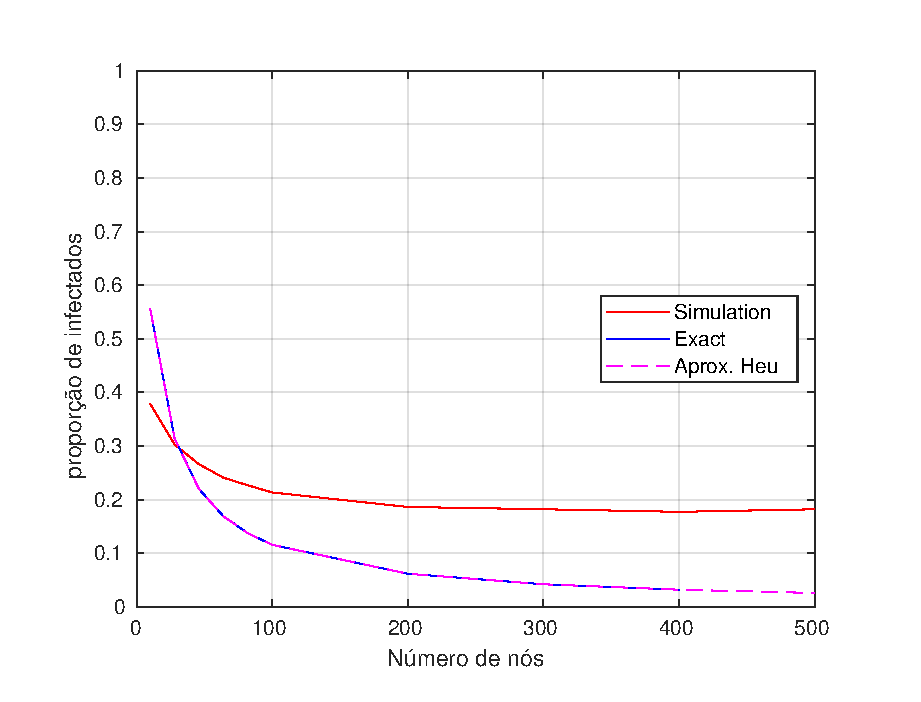
\includegraphics[width=0.35\columnwidth]{img/fig_i_3000_v0_lambda1500_mu122_9877_gamma1_006100_iter_2_rho0_0.pdf}\\
	        (a) $\alpha = 8 \times 10^{-5}$ & 
	        (b) $\beta  = 5 \times 10^{-2}$ & 
	        (c) $\tau   = 18$\\
	        $\mu = 17.959$, $\gamma = 1.0071$ &
            $\mu = 154.888$, $\gamma = 1.0262$ &
            $\mu = 122.987$, $\gamma = 1.0061$\\
	        %------------------------------------------------------
	        \hspace{-0.6cm}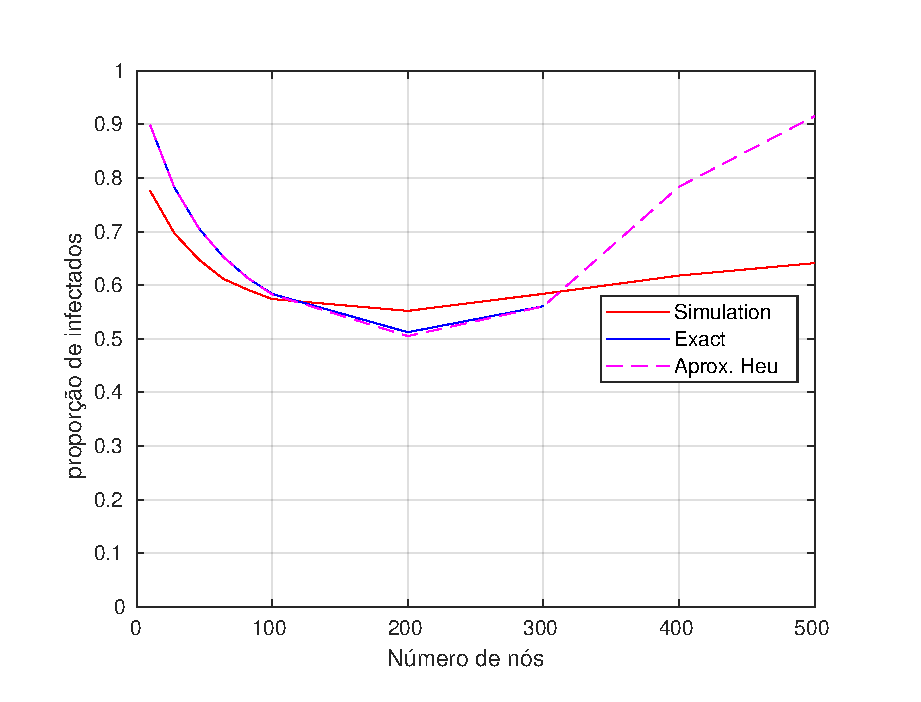
\includegraphics[width=0.35\columnwidth]{img/fig_b_1001_v0_lambda1500_mu18_1603_gamma1_009200_iter_2_rho0_0.pdf} & 
	        \hspace{-0.6cm}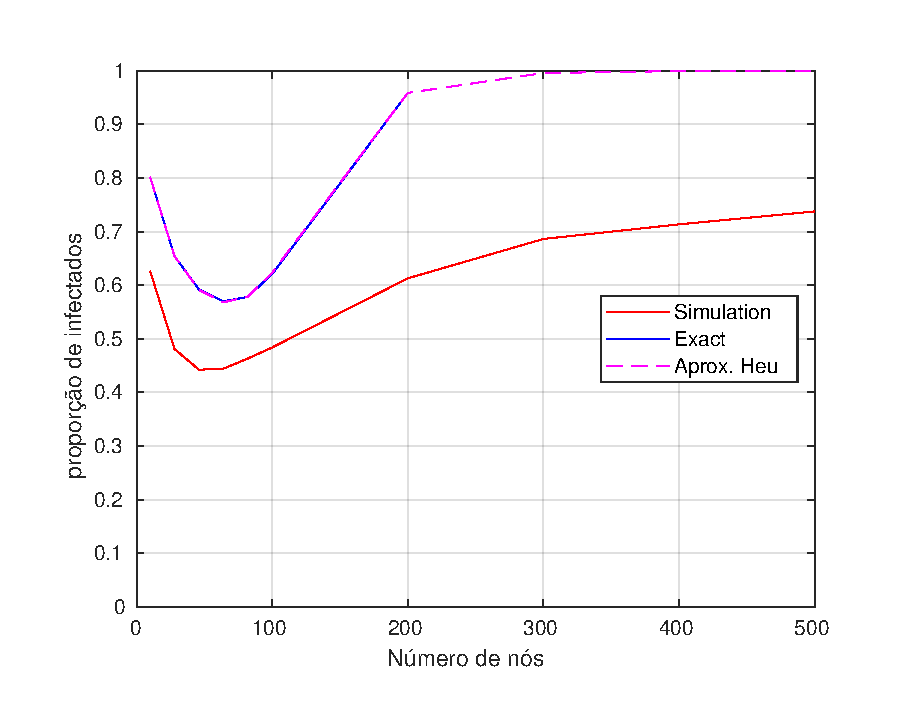
\includegraphics[width=0.35\columnwidth]{img/fig_f_2001_v0_lambda1500_mu44_7099_gamma1_026200_iter_2_rho0_0.pdf} &
	        \hspace{-0.6cm}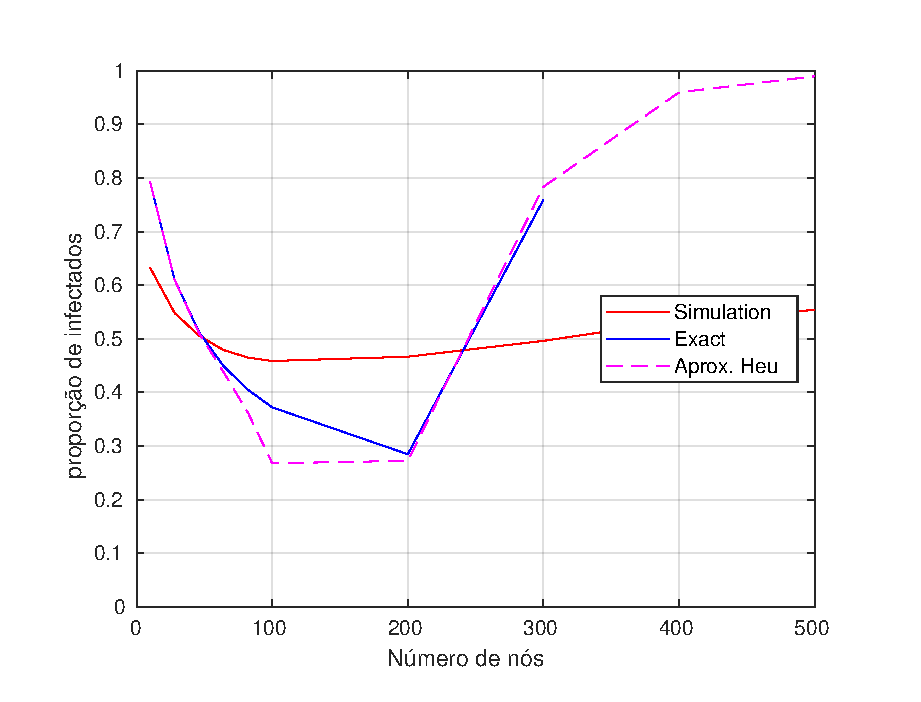
\includegraphics[width=0.35\columnwidth]{img/fig_j_3001_v0_lambda1500_mu43_5209_gamma1_014800_iter_2_rho0_0.pdf}\\
	        (d) $\alpha = 20 \times 10^{-5}$ & 
	        (e) $\beta  = 32 \times 10^{-2}$ & 
	        (f) $\tau   = 40$\\
	        $\mu = 18.160$, $\gamma = 1.0092$ &
            $\mu = 44.710$, $\gamma = 1.0262$ &
            $\mu = 43.521$, $\gamma = 1.0148$ \\
	        %------------------------------------------------------
	        \hspace{-0.6cm}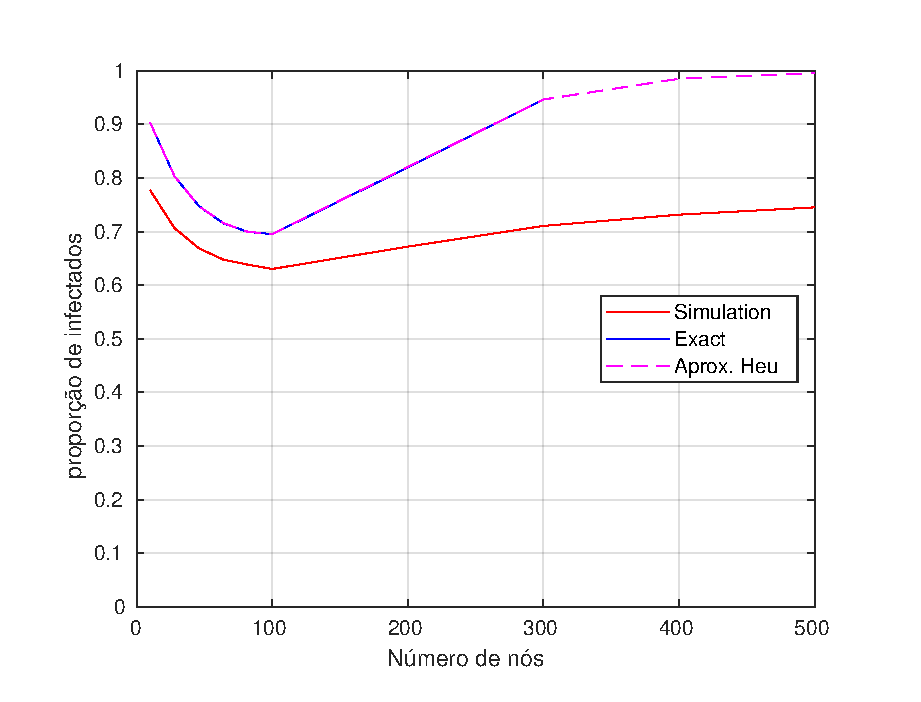
\includegraphics[width=0.35\columnwidth]{img/fig_c_1002_v0_lambda1500_mu18_0462_gamma1_014800_iter_2_rho0_0.pdf} & 
	        \hspace{-0.6cm}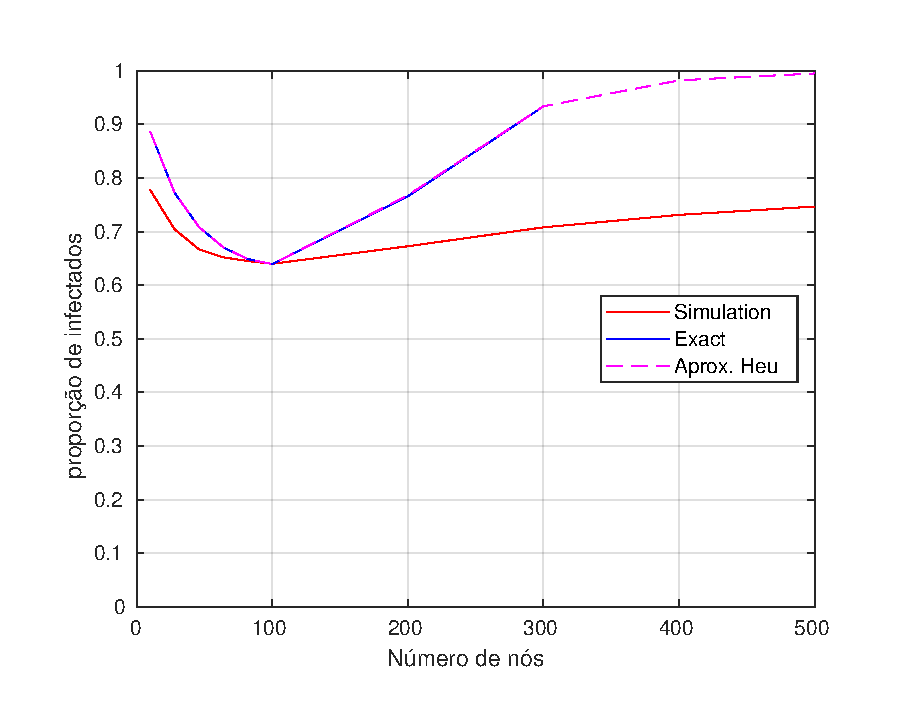
\includegraphics[width=0.35\columnwidth]{img/fig_g_2002_v0_lambda1500_mu21_4111_gamma1_014800_iter_2_rho0_0.pdf} &
	        \hspace{-0.6cm}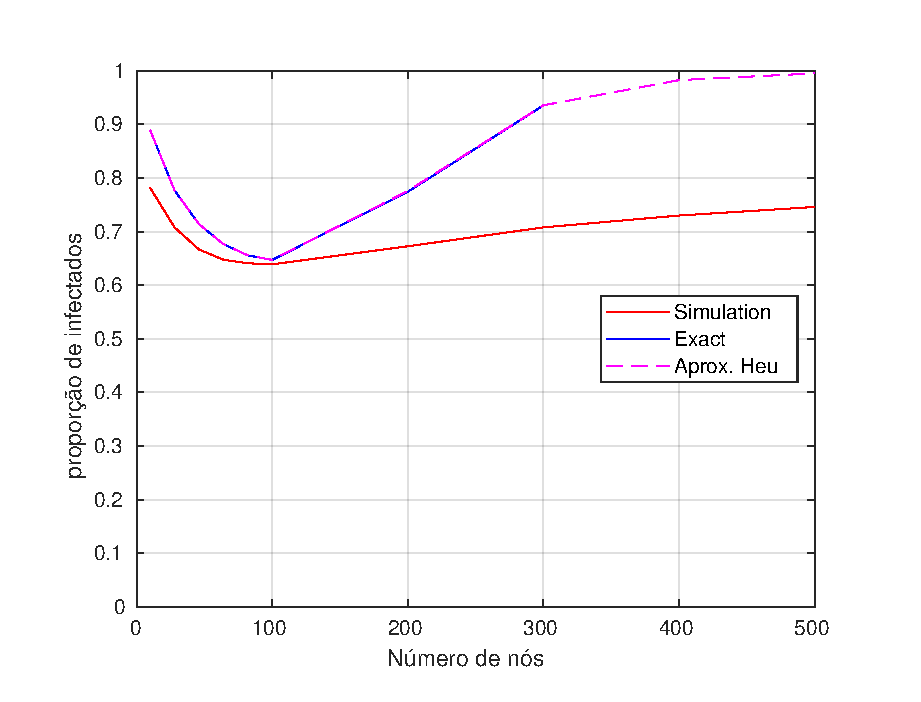
\includegraphics[width=0.35\columnwidth]{img/fig_k_3002_v0_lambda1500_mu20_9333_gamma1_014800_iter_2_rho0_0.pdf}\\
	        (g) $\alpha = 50 \times 10^{-5}$ & 
	        (h) $\beta  = 200 \times 10^{-2}$ & 
	        (i) $\tau   = 65$\\
	        $\mu = 18.046$, $\gamma = 1.0148$ &
            $\mu = 15.717$, $\gamma = 1.0071$ &
            $\mu = 2.882$, $\gamma = 1.0171$ \\
	        %------------------------------------------------------
	        \hspace{-0.6cm}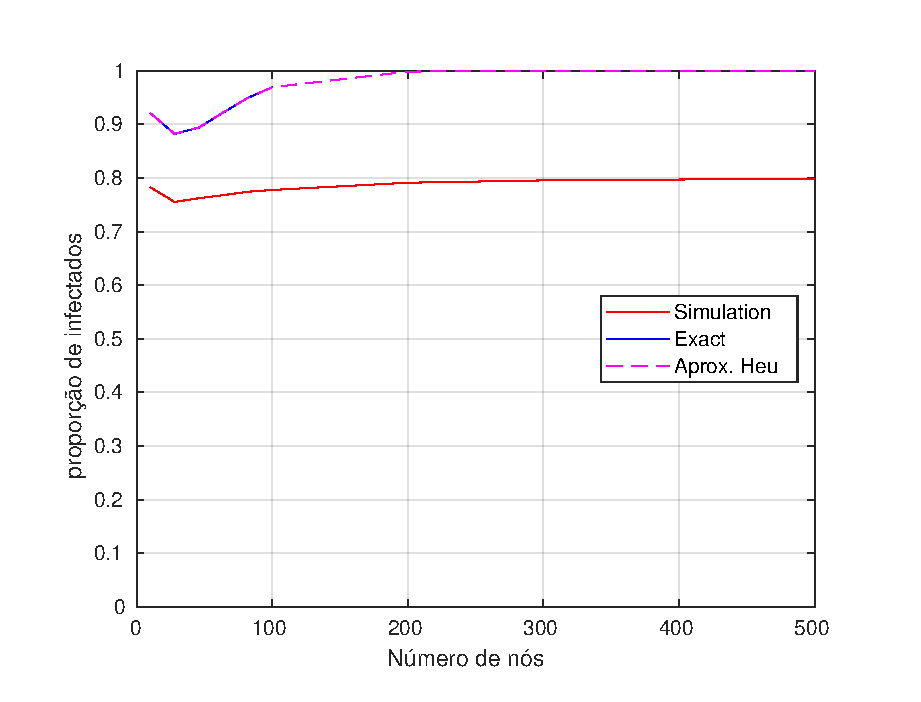
\includegraphics[width=0.35\columnwidth]{img/fig_d_1003_v0_lambda1500_mu17_4592_gamma1_038300_iter_2_rho0_0.pdf} & 
	        \hspace{-0.6cm}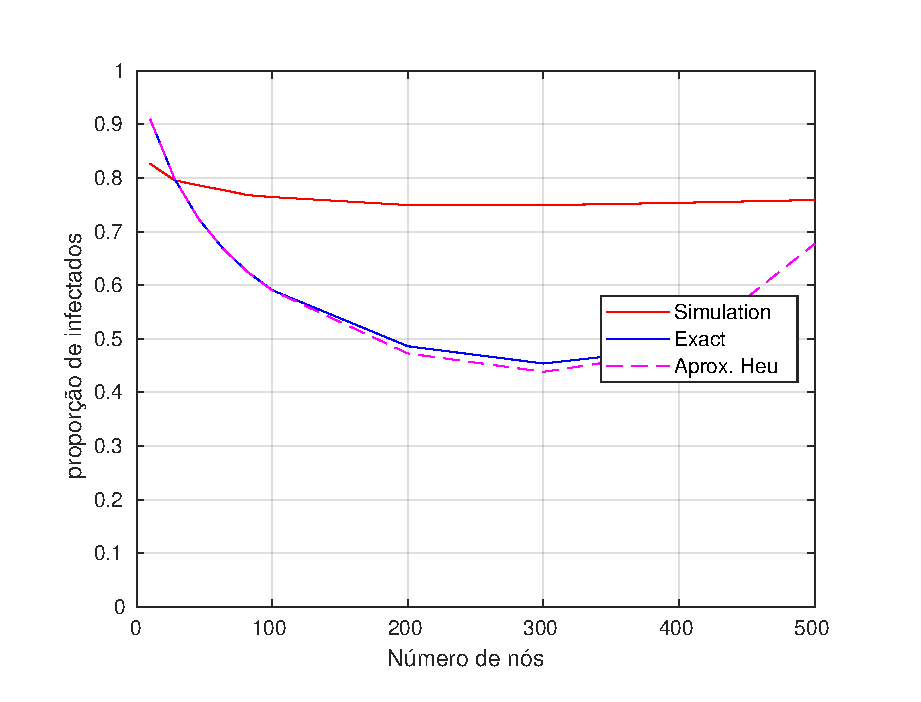
\includegraphics[width=0.35\columnwidth]{img/fig_h_2003_v0_lambda1500_mu15_7172_gamma1_007100_iter_2_rho0_0.pdf} &
	        \hspace{-0.6cm}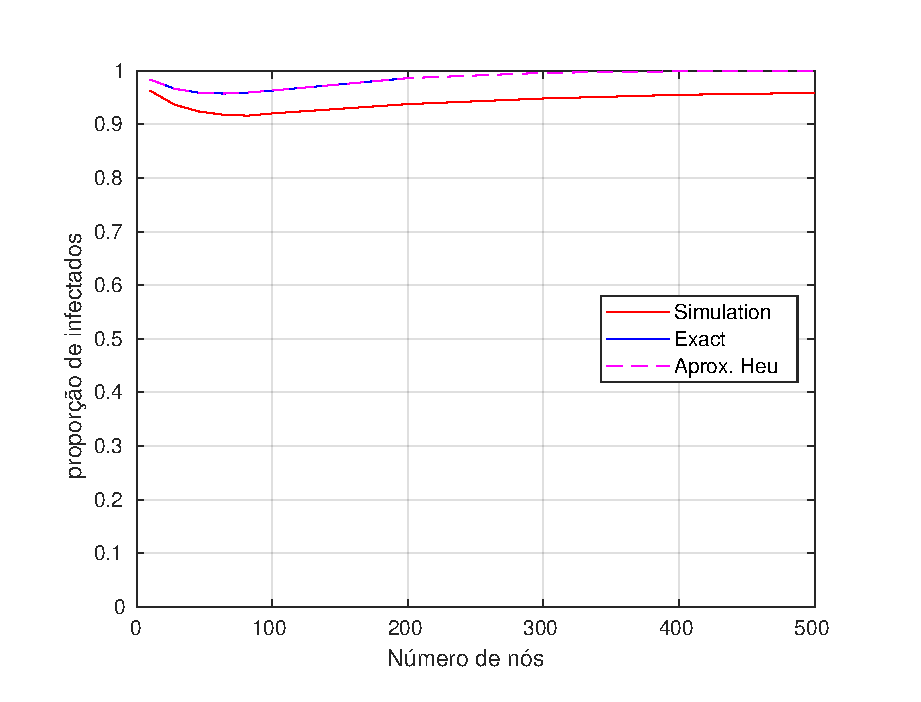
\includegraphics[width=0.35\columnwidth]{img/fig_l_3003_v0_lambda1500_mu2_8819_gamma1_017100_iter_2_rho0_0.pdf}\\
	        (j) $\alpha = 500 \times 10^{-5}$ & 
	        (k) $\beta  = 2000 \times 10^{-2}$ & 
	        (l) $\tau   = 260$ \\
	        $\mu = 17.459$, $\gamma = 1.0383$ &
            $\mu = 21.411$, $\gamma = 1.0148$ &
            $\mu = 20.933$, $\gamma = 1.0148$ 
	        %------------------------------------------------------
	    \end{tabular}
	    \caption{Resultados de simulação para o comportamento da rede totalmente conectada, sob atuação da \textit{Botnet Mirai}  na presença de um atacante estratégico.  Modelo analítico da Seção~\ref{sec:fechadageral} parametrizado com $\Lambda = 1500$ e valores adicionais indicados na figura. }
	    \label{fig:simulacao_resultados_1a_parte}
	\end{figure}
	
	
	
		\textbf{Modelo analítico e simulação}  A Fig.~\ref{fig:simulacao_resultados_1a_parte}  ilustra a probabilidade de infecção segundo o modelo analítico proposto (tanto solução exata quanto  aproximada, nas curvas rosa e azul, respectivamente).   O modelo captura qualitativamente o comportamento da simulação, indicando que no regime inicial, quando o número de nós na rede é pequeno, o sistema é dominado por infecções exógenas.  Na medida em que o número de nós na rede aumenta, a probabilidade de infecção primeiro diminui e depois aumenta, atingindo o segundo regime no qual   o sistema é dominado por infecções endógenas.  
		
	Em geral, o modelo tende a superestimar a probabilidade de infecção em relação à simulação.  Isto deve-se ao fato de que $(i)$ no modelo assumimos que os nós estão sempre ligados, enquanto que na simulação os nós alternam entre ligados e desligados,   $(ii)$  o modelo assume contribuições multiplicativas das taxas de infecção, enquanto que a simulação considera contribuições aditivas e $(iii)$  no modelo, todos os tempos entre eventos são exponencialmente distribuídos, enquanto que na simulação a latência na rede é uniforme (tal latência não é levada em conta no modelo).  Trabalhos futuros consistem em verificar sob que condições o modelo  produz um limite superior para a probabilidade de infecção de fato observada na rede.   Note também que embora a aproximação proposta tenha apresentado bons resultados na Figura~\ref{fig:rho_exact_approx_newton_rho0_0e1}, em alguns cenários da Figura~\ref{fig:simulacao_resultados_1a_parte} a aproximação distanciou-se do valor exato previsto pelo modelo, e estamos no momento averiguando formas de refinar a aproximação.  
	
	    
	    \textbf{Análise de sensitividade} Para estudar a sensitividade da probabilidade de infecção em função dos diferentes parâmetros do sistema, mantemos todos os parâmetros fixos e variamos um de cada vez para avaliar seu impacto.   Em particular, na primeira, segunda e terceira colunas da Figura~\ref{fig:simulacao_resultados_1a_parte} variamos a taxa de contaminação endógena ($\alpha$), taxa de contaminação exógena ($\beta$) e tempo médio que o dispositivo permanece ligado ($\tau$). Nas curvas obtidas via simulação indicamos o intervalo de confiança de $95\%$.   As linhas roxa e verde correspondem, respectivamente, à solução exata do modelo (eq.~\eqref{eq:scaledSISProbIotaInfected}) e à aproximação de Newton, com duas iterações, conforme  heurística definida na Seção~\ref{subsec:heuristica}. 
	     \emph{Cabe ressaltar que o simulador caracteriza detalhadamente o  comportamento do \textit{Mirai Botnet}, enquanto  o modelo proposto  captura a essência do  sistema.}
	    
\emph{O sistema passa por dois regimes fundamentais, primeiro sendo dominado por infecções endógenas e depois por infecções exógenas. }	    Em todos os cenários apresentados na Figura~\ref{fig:simulacao_resultados_1a_parte} observa-se  que o sistema passa por dois regimes.  Tal fato pode ser constatado focando-se nas linhas pontilhadas e tracejadas, que crescem e diminuem, respectivamente,  na medida em que o número de nós no sistema aumenta.   Tal comportamento observado em simulações está de acordo com o previsto pelas equações~\eqref{eq:mainlema1} e \eqref{eq:newton_general}.  No primeiro regime, o sistema é dominado por infecções exógenas (linha tracejada  acima da linha pontilhada).  Na medida em que o número de nós na rede aumenta, as infecções endógenas também passam a exercer papel  importante.  No segundo regime, o sistema é dominado por infecções endógenas (linha tracejada  acima da linha pontilhada).  Em nossas simulações, observamos que o número de nós no sistema correspondente ao cruzamento dos gráficos de infecções endógenas e exógenas (cruzamento das curvas pontilhada e tracejada) é igual ou aproximadamente igual  a aquele que minimiza a  proporção de nós infectados (curva vermelha).
	    
	    
	    
\emph{A probabilidade de infecção é mais sensível à taxa de contaminação endógena  que à taxa de contaminação exógena. } Isto ocorre porque a taxa de infecção endógena é amplificada pelo número de nós infectados na rede, enquanto que a taxa de infecção exógena é limitada pelo \emph{Botmaster}.  Um aumento em torno de $60$ vezes da taxa de infecção endógena produz os efeitos observados na primeira coluna da Figura~\ref{fig:simulacao_resultados_1a_parte}.  Já  a taxa de infecção exógena teve um aumento de $400$ vezes para observarmos a variação de  padrões na segunda coluna da  Figura~\ref{fig:simulacao_resultados_1a_parte}.
	    

	    
	    \emph{O tempo médio que um dispositivo não vacinado permanece ligado (logo, suscetível) é também um fator relevante na simulação.} O valor  assintótico da fração de nós infectados, por exemplo, depende do tempo médio que um dispositivo permanece ligado, conforme vemos na última coluna da Figura~\ref{fig:simulacao_resultados_1a_parte}.   Na medida em que os nós permanecem mais tempo ligados, a proporção de nós infectados também aumenta. \emph{ Simplesmente desligar os sistemas pode ser uma estratégia eficaz para conter epidemias. Entretanto, tal estratégia pode acabar por atender aos anseios do atacante, de causar um ataque de DDoS por indisponibilidade dos sistemas alvos.}
	    

% ---------------------------------------------------------
% Análise do Modelo
% ---------------------------------------------------------

% ---
% Análise do Modelo
% ---
\chapter{Análise do Modelo}
\label{cap:analise}
% ---
    \section{Análise do modelo} 
    \label{sec:model_analysis}
	    A seguir, focamos em uma topologia totalmente conectada. Neste caso, por simetria temos que
        \begin{align}
            \tilde{\pi}(i) &= \binom{N}{i}  \left( \frac{\lambda(N)}{\mu} \right)^{i} \gamma^{i(i-1)/2}, \quad i=0, \ldots, N
        \end{align}
    	A probabilidade de infecção de um nó aleatório escolhido de uma distribuição uniforme dos nós:
    	\begin{equation}
    		{\rho}(N) = \frac{1}{N}    \sum\limits_{i=0}^{N} i \frac{\tilde{\pi}(i)}{{Z}}  
    		\label{eq:rho_N}
    	\end{equation}
	    A análise direta das equações acima é complexa, por envolver um termo quadrático no expoente de $\gamma$.  Para simplificar a análise,  consideramos  uma solução aproximada para o modelo acima. Para tal, definimos $\hat\rho(N) \approx \rho(N)$ e $\hat\pi(i) \approx \tilde\pi(i)$, 
	    \begin{align}
            \hat{\rho}(N) &= \frac{1}{N} \sum\limits_{i=0}^{N} i \frac{\hat{\pi}(i)}{{\hat Z}}\label{eq:rho_Nhat2} \\
            \hat{\pi}(i)  &= \binom{N}{i} \left(\frac{\lambda(N)}{\mu}\gamma^{N^{\star}/2}\right)^{i} \label{eq:tilde_pi_i} \\
            \hat{Z} &= \sum\limits_{i=0}^{N} \hat{\pi}(i) \label{eq:tilde_hat_z}
        \end{align}
		onde $N^{\star}(N)$ é uma função crescente de $N$, que denotamos simplesmente por $N^{\star}$ para simplificar a notação.  Nos referimos a o modelo proposto para aproximar a solução do modelo original como \textit{aproximação binomial}, por fazermos uso do binômio de Newton na demonstração do resultado a seguir: 

        \begin{lemma}
        No modelo binomial,  temos que 
        	\begin{equation}
				\hat{\rho}(N) =   \frac{1}  {1+ \mu/(\lambda(N) \gamma^{N^{\star}/2} )  } \\
        	\end{equation}
        \end{lemma}	
        \begin{proof}	
            O resultado é fruto de manipulações algébricas,
            \begin{align}
            \hat{Z} \hat{\rho}(N) &= \frac{1}{N} \sum_{i=0}^N i \binom{N}{i} \left( \frac{\lambda(N)}{\mu}\gamma^{N^{\star}/2} \right)^i = \sum_{i=1}^N\binom{N-1}{i-1}\left(\frac{\lambda(N)}{\mu}\gamma^{N^{\star}/2}\right)^i \label{eq:binom_mirror} \\
            &= \color{black}{\left(\frac{\lambda(N)}{\mu}\gamma^{N^{\star}/2}\right)\left(1+\frac{\lambda(N)}{\mu}\gamma^{N^{\star}/2}\right)^{N-1}} \label{eq:thm_binom} %\tag{3}
            \end{align}
            O resultado segue a partir da obtenção, de forma similar, da  expressão de $\hat{Z}$. 
        \end{proof}
        O resultado acima pode ser usado, por exemplo, para caracterizarmos os pontos de equilíbrio do sistema.

        \begin{thm}
            O modelo binomial admite no máximo dois equilíbrios interiores ao considerarmos um custo de vacinação constante, desde que $\gamma>1$, $\partial N^{\star}/\partial N$ seja positivo e não decrescente e $\lambda(N)$ decrescente.     \label{thm:main}
        \end{thm}
        \begin{proof}
            Seja $\tau(N)= (\lambda(N)/\mu)\gamma^{N^{\star}/2}$. Então, pelo lema acima, temos que $\partial \hat \rho(N)/\partial N =  (\partial \tau/\partial N)/(\tau^2 (1+1/\tau)^2)$. Claramente, todos os termos de $\partial \hat \rho(N)/\partial N$ são positivos, com exceção de $\partial \tau/\partial N$.  Temos que
            \begin{equation}
            \frac{\partial \tau}{\partial N} = \lambda(N) \gamma^{N^{\star}/2} \left(\frac{1}{2} \log \gamma  \frac{\partial N^{\star}}{\partial N} + \frac{\lambda'(N)}{\lambda(N)}   \right)
            \end{equation}
            Se $ \frac{\partial N^{\star}}{\partial N} $ for positivo e não decrescente, e $\lambda(N)$  for decrescente, a expressão acima admite um único zero.  Assim, a função $\hat \rho(N)$ possui no máximo um ponto de mínimo interno, e por isso cruza qualquer linha horizontal em no máximo dois pontos.   
        \end{proof}
        O resultado acima está de acordo com a ilustração apresentada nas Figuras~\ref{fig:result_01b}~e~\ref{fig:equilibrim_cost}. Segundo a Figura~\ref{fig:result_01b}, em todos os casos em que $\gamma > 1$, a probabilidade de um nó estar infectado primeiro diminui e depois aumenta, ou simplesmente sempre aumenta.  Conforme discutido na Figura~\ref{fig:equilibrim_cost}, a um ponto de mínimo correspondem dois equilíbrios, um estável e um instável. 

        \paragraph*{Caso especial: $\lambda(N)=\Lambda/N$}
        O modelo proposto é factível de análise em fórmula fechada para vários casos especiais da função $\lambda(N)$. Para fins de ilustração, consideramos o caso especial em que $\lambda(N)=\Lambda/N$.  Este caso corresponde a um atacante que tem poder de ataque (\emph{budget}) constante igual a $\Lambda$ infecções por segundo, e divide esse poder entre os $N$ nós da rede. Nesse caso, $\lambda' (N) = -\Lambda/N^2$. Assumindo para fins de simplificação que  $N^{\star}=N$, temos
		\begin{equation}
			\frac{\partial}{\partial N}\hat{\rho}(N)  = \kappa \left( \frac{1}{2} \log \gamma - \frac{1}{N} \right)
		\end{equation}
		onde $\kappa$ é uma constante positiva. 
		Podemos verificar que $\frac{\partial}{\partial N}\hat{\rho}(N)=0$ quando $N = (2 / \log \gamma)$. % para valores $N < (2 / \log \gamma)$ a derivada é negativa, e valores $N > (2 / \log \gamma)$ a derivada é positiva. 
		No caso de $\gamma = 1.09$ encontramos o valor crítico quando $N \approx 23$, que está de acordo com aquele apresentado na Figura~\ref{fig:result_01b}. 

        Note também que podemos obter fórmulas fechadas para os pontos de equilíbrio.
        Para tal, seja $C$ o custo de aplicação da contramedida.  Então, os pontos de equilíbrio interno são pontos tais que $\hat{\rho} (N) - C = 0$. 
		Assumindo para fins de simplificação que  $N^{\star}=N$, temos que 
		os valores de $N$ que satisfazem a equação de equilíbrio são  
		$N = \frac{-2}{\log \gamma}    W \left(\frac{\Lambda (C-1) \log\gamma}{2C \gamma^{1/2} }  \right)$ 
		onde $W(x)$ é a função de Lambert, que admite dois valores reais, correspondentes aos ramos -1 e 0.  
		No caso de $\Lambda = 10$, $\gamma = 1,09$ e $C = 0.6$, por exemplo, temos os valores de $N$ correspondentes aos ramos $-1$ e $0$  dados por 45,6 e  9,7.  O segundo equilíbrio condiz com o  resultado da   Figura~\ref{fig:equilibrim_cost}, enquanto que o primeiro foi superestimado. Tal fato deve-se à simplificação de que $N^{\star}=N$, conforme ilustrado na Figura~\ref{fig:result_01b}, podendo o resultado ser melhor aproximado em refinamentos sucessivos do modelo. 
		A Figura~\ref{fig:result_01b}(a) mostra a probabilidade de um nó estar infectado, em função do número de nós na rede.  A aproximação $N^{\star}=N$ captura bem o comportamento do sistema antes de $\rho(N)$ atingir o seu ponto de mínimo. Depois deste ponto, é necessário ajustar $N^{\star}$ para o seu valor ótimo, que é crescente e sempre maior que $N$ como ilustrado na Figura~\ref{fig:result_01b}(b) (satisfazendo os critérios do Teorema ~\ref{thm:main}).  
		De forma mais geral, cabe destacar que o fato de a   função de Lambert possuir dois ramos reais  está de acordo com a constatação de que o sistema admite  no máximo dois equilíbrios internos (vide Teorema~\ref{thm:main}).   

        \begin{figure}[!htb]
    		\centering
    	    \hspace{-0.2in}	
            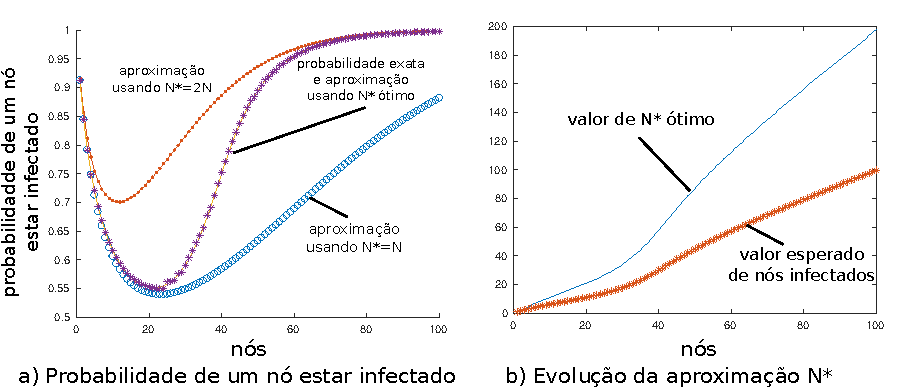
\includegraphics[width=0.99\columnwidth,keepaspectratio=false]{./img/aproximacoes_N_ast.pdf}
    		\caption{Validação da solução aproximada pelo modelo binomial ($\gamma=1,09$).}
    		\label{fig:result_01b}
        \end{figure}
        
        

% ---------------------------------------------------------
% Trabalhos relacionados

% ---
% Trabalhos Relacionados
% ---
\chapter{Trabalhos Relacionados}
\label{cap:trab_relac}
% ---



A literatura sobre modelos epidemiológicos é vasta, levando em conta aspectos transientes~\cite{ganesh2005effect} e estacionários~\cite{keeling2005networks, ratton}, bem como infecções endógenas e exógenas~\cite{zhang2017contact,zhang2015Network,zhang2018more}. Entretanto, não é de nosso conhecimento nenhum trabalho  que tenha analisado modelos analíticos levando em consideração atacantes estratégicos, de capacidade limitada, capazes de causar infecções exógenas, gerando expressões para a probabilidade de infecção dos nós.


Este trabalho é uma extensão de~\cite{rufino2018contaminaccao}.  Em~\cite{rufino2018contaminaccao} propusemos o modelo epidemiológico analisado no presente artigo.  Dentre as principais contribuições do presente trabalho, que não constavam em~\cite{rufino2018contaminaccao}, destacamos três: $(i)$ aproveitando-se de resultados recentes apresentados em~\cite{zhang2018more}, derivamos um método iterativo  para calcular a probabilidade de infecção dos nós.  Em seguida, apresentamos $(ii)$   fórmulas fechadas para aproximar a probabilidade de infecção assim como   $(iii)$   resultados de simulação. 

A proliferação de \emph{malware} e a formação de grandes \emph{botnets} permitem a execução de ataques distribuídos de negação de serviço com volume capaz de afetar serviços com grande capacidade \cite{kolias2017ddos, dynddos}. O crescimento da Internet das Coisas (IoT)~\cite{peterson}, combinado com as vulnerabilidades presentes nestes dispositivos e a dificuldade de atualizá-los criaram um ambiente propício para construção de \emph{botnets} \cite{angrishi2017turning}.  
As caracterizações e comportamentos observados em \emph{malware} real podem ser utilizados para parametrizar nossos modelo e simulador. Nossos modelos e o simulador são gerais o suficiente para serem  aplicados a novos \emph{malwares} que venham a ser identificados e caracterizados.   


Vários trabalhos na literatura estudam o comportamento e a evolução de \emph{malwares} \cite{antonakakis2017understanding, marzano2018evolution}.  Existe uma  constante evolução dos \emph{malwares} por parte dos atacantes.  \emph{Assim, a transição do estado infectado para o estado  suscetível  considerada neste trabalho pode refletir o fato de que um nó infectado, após aplicar uma contramedida, voltou a se tornar suscetível com relação a novas variantes de um mesmo \emph{malware}.} 






% ---------------------------------------------------------
% Cronograma

% ---
% Cronograma de Trabalho
% ---
\chapter{Cronograma de trabalho}
\label{cap:cronograma}
% ---
O restante do trabalho será desenvolvido em cotutela com a \textit{Université d’Avignon}, onde nossos resultados serão incrementados com desenvolvimento de formulações matemáticas que auxiliem a caracterização de medidas de centralidade em redes, com interesse em segurança da informação.

\textbf{Atividades em conjunto com a ``Université d’Avignon''}:
\begin{enumerate}
    \item \textbf{2019 - MAI:} Revisão das definições e metodologias de centralidades em redes;
    \item \textbf{2019 - JUN:} Desenvolvimento das formulações matemáticas de interesse para o problema de Segurança da Informação \label{enum:jun2019};
    \item \textbf{2019 - JUL} Implementação da primeira solução, usando a metodologia desenvolvida em \ref{enum:jun2019};
    \item \textbf{2019 - AGO} Validação dos resultados com o mundo real, usando-se dados públicos ou dados simulados;
    \item \textbf{2019 - SET} Submissão de trabalho científico.
    \item \textbf{2019 - OUT} Revisar os experimentos com possíveis dados locais, possivelmente com a integração dos trabalhos;
    \item \textbf{2019 - NOV e DEZ} Realização de experimentos computacionais;
    \item \textbf{2020 - JAN} Submissão de trabalho científico;
    \item \textbf{2020 - FEV e MAR} Escrita de Tese e revisão pelos orientadores;
    \item \textbf{2020 - ABR} Submissão de Tese;
    \item \textbf{2020 - MAI} Defesa de Tese.
\end{enumerate}

% ---------------------------------------------------------

% ----------------------------------------------------------
% Não usado no modelo UFRJ
% Finaliza a parte no bookmark do PDF
% para que se inicie o bookmark na raiz
% e adiciona espaço de parte no Sumário
% ----------------------------------------------------------
%\phantompart

% ---------------------------------------------------------
% Conclusões
% ---------------------------------------------------------

% ---
% Conclusão
% ---
\chapter{Conclusão}
\label{cap:conclusao}
% ---


Neste trabalho, consideramos a  caracterização do processo de propagação de epidemias frente atacantes estratégicos. Em particular, considerando o modelo analítico previamente proposto em~\cite{rufino2018contaminaccao, rufino2019dilemas},  propusemos um método iterativo para calcular a probabilidade de infecção dos nós.   Comparando os resultados analíticos  com resultados de simulações, observamos que o modelo captura o comportamento do sistema mesmo quando consideramos nós intermitentes, bem como tempos entre eventos que não sejam exponencialmente distribuídos. Acreditamos que os resultados apresentados neste artigo constituam um passo no sentido de estabelecer os fundamentos para melhor modelagem e análise   do processo de propagação de epidemias.  Tal entendimento é crítico para auxiliar na tomada de decisões, por exemplo, sobre vacinar ou reiniciar sistemas conectados à rede, levando em conta os custos de tais contramedidas e os respectivos riscos da não implementação das mesmas.

% ---------------------------------------------------------


% ------------------------------------------------------------------------
% FIM ELEMENTOS TEXTUAIS
% ------------------------------------------------------------------------
% ------------------------------------------------------------------------
% ------------------------------------------------------------------------

% ------------------------------------------------------------------------
% ------------------------------------------------------------------------
% ------------------------------------------------------------------------
% ELEMENTOS PÓS-TEXTUAIS
% ------------------------------------------------------------------------
\postextual

% ------------------------------------------------------------------------
% REFERÊNCIAS BIBLIOGRÁFICAS 
\bibliography{1000_bibliograf}

% ----------------------------------------------------------
% GLOSSÁRIO
% Consulte o manual da classe abntex2 para orientações sobre o glossário.
%\glossary

% ----------------------------------------------------------
% APÊNDICES
% Texto ou documento elaborado pelo autor, 
% a fim de complementar sua argumentação, sem prejuízo da 
% unidade nuclear do trabalho
%
% ----------------------------------------------------------
% Apêndices
% ----------------------------------------------------------

% ---
% Inicia os apêndices
% ---
\begin{apendicesenv}

% Imprime uma página indicando o início dos apêndices
\partapendices

% ----------------------------------------------------------
\chapter{Quisque libero justo}
% ----------------------------------------------------------

\lipsum[50]

% ----------------------------------------------------------
\chapter{Nullam elementum urna vel imperdiet sodales elit ipsum pharetra ligula
ac pretium ante justo a nulla curabitur tristique arcu eu metus}
% ----------------------------------------------------------
\lipsum[55-57]

\end{apendicesenv}

% ----------------------------------------------------------
% ANEXOS
% Texto ou documento não elaborado pelo autor, que serve de 
% fundamentação, comprovação e ilustração
%
% ----------------------------------------------------------
% Anexos
% ----------------------------------------------------------

% ---
% Inicia os anexos
% ---
\begin{anexosenv}

% Imprime uma página indicando o início dos anexos
\partanexos

% ---
\chapter{Morbi ultrices rutrum lorem.}
% ---
\lipsum[30]

% ---
\chapter{Cras non urna sed feugiat cum sociis natoque penatibus et magnis dis
parturient montes nascetur ridiculus mus}
% ---

\lipsum[31]

% ---
\chapter{Fusce facilisis lacinia dui}
% ---

\lipsum[32]

\end{anexosenv}

%---------------------------------------------------------------------
% INDICE REMISSIVO
\phantompart
\printindex
% ------------------------------------------------------------------------
% FIM ELEMENTOS PÓS-TEXTUAIS
% ------------------------------------------------------------------------
% ------------------------------------------------------------------------
% ------------------------------------------------------------------------

\end{document}